\chap{Group Actions}{actions}
We've defined a  ``group'' as as set with an operation defined on it.  From this point of view, group elements are ``objects'' in a set. We have many examples of this: like the integers with addition, the integers mod $n$, the group of units $U(n)$, groups of matrices, and so on.

Later on we introduced the idea that permutations form a group. Permutations are actually bijections (1-1, onto functions) that map a set of objects to itself.  Another way of saying this is that permutations ``act on'' a set by moving the elements around.  Similarly, we saw in Figure~\ref{groups_s3_symmetry_fig} in Section~\ref{SymmetryGroup} that the symmetries of an equilateral triangle (which are elements of the group $S_3$) move the vertices of the triangle from one position to another.  As a third example, in the group $\mathbb {Q}^*$ of non-zero rational numbers we can think of left multiplying by $2$ as ``moving''  $-5$ over to $-10$.  Left multiplying again by $2$ ``moves'' $-10$ to $-20$: and so on.   

The examples in the previous paragraph  illustrate a general concept called \emph{group actions}\index{Actions!group}. We will see in this chapter how group actions can give us deeper insight into many of the symmetries that we see in the world around us: for instance, in the geometric solids and in crystals.\footnote{This chapter  is by Holly Webb (edited by C.T.). Thanks to Tom Judson for material used in this chapter.}

\section {Basic definitions}\label{DefActions}
We'll get to definitions momentarily, but first it's helpful to look at one more example.

\begin{example}{Actions1} 
Consider the $60^{\circ}$ counterclockwise rotation of regular hexagon, an element of the group $D_6$.  We've seen this before (see Example~\ref{example:symmetries:hexagon} in Chapter~\ref{symmetries}). Following are the tableau and cycle representations of this rotation. 
\[ \text{tableau:}~~r_{60} = \begin{pmatrix} A & B & C & D & E & F \\ B & C & D & E & F  & A \end{pmatrix}; \qquad 
\text{cycle:}~~r_{60}=(A B C D E F).\]
 Both these notations indicate that the rotation acts on the set of vertices (by producing a permutation).  In the same way, any symmetry of the hexagon (rotation or reflection) acts on vertices of the hexagon.
\end{example}
	\begin {exercise}{Actions2}  Generalize the previous example to any regular $n$-gon. Include a tableau in your answer.
\end {exercise}
Now we're ready to give a general definition of group action. 

\begin{defn}
Let $X$ be a set and $G$ be a group. A \bfii{(left) action}\index{Actions!group} of $G$ on $X$ is a map $G\times X\rightarrow X$
given by $(g, x)\rightarrow gx$, where
\begin{enumerate}[(1)]
\item $ex = x$ for all $x\in X$;
\item $(g_1g_2)x = g_1(g_2x)$ for all $x\in X$ and all $g_1, g_2 \in G$.
\end{enumerate}
The set $X$  on which $G$ acts is called a  \bfii{$G$-set}.\index{$G$-set}
\end{defn}
It is also possible to define right group actions, but in this chapter we'll focus just on left group actions.\index{Actions!left and right}  Following are some more examples of group actions.

\begin{example}{Actions3}
 Let $G = GL_2(\mathbb{R})$ (the group of invertible $2 \times 2$ matrices) and $X = \mathbb{R}^2$
Then $G$ acts on $X$ by left multiplication. If $v\in \mathbb{ R}^2$
and $I$ is the identity matrix, then $Iv = v$. If $A$ and $B$ are $2 \times 2$
invertible matrices, then $(AB)v = A(Bv)$ since matrix multiplication is associative.  Therefore, by definition, $X$ is a $G$-set.\end{example}

\begin {exercise}{Actions4}
Let
\begin{equation*}
A=\left[\begin {array}{cc}
a&b\\c&d\end{array}\right]; \quad 
B=\left[\begin{array}{cc} e& f\\ g & h\end{array}\right]; \quad 
v=\left[\begin{array}{c}x\\ y\end{array}\right].
\end{equation*}
Verify the previous example by showing associative property of matrix and vector multiplication. 
\end {exercise}

\begin{exercise}{Action5}
\begin{enumerate}[(a)]
\item 
Let $G = 2\mathbb{Z}$ and let $X =\mathbb{Z}$. Show that $X$ is a $G$-set.
\item Let $G = \mathbb{Z}$ and let $X = 2\mathbb{Z}$. Is $X$ a $G$-set? Explain.
\item Let $G = H_6$ (the complex $6$-th roots of unity (see Section~\ref{sec:RootsOfUnity} in Chapter~\ref{complex}) and let $X =\mathbb{C}$. Show that $X$ is a $G$-set.
\item Let $G = \mathbb{C}$ and let $X = H_8$.  Is $X$ a $G$-set? Explain.
\end{enumerate}
\end{exercise}
\section{Group actions on regular polyhedra}\label{ActionsOnPolyhedra}
We want to apply our new ideas to gain insight about the groups of rotational symmetries of \bfii{regular polyhedra}\index{Polyhedron!regular}  In general, a \emph{polyhedron} can be thought of as a collection of faces, edges and vertices: for example, a cube has 6 faces, 12 edges and 8 vertices. A\emph{regular polyhedron} is a polyhedron in which all faces are congruent regular polygons, and the same number of edges meet at every vertex. The group of rotational symmetries of a polyhedron act on the faces, edges and vertices.  A rotation will always take faces to faces, edges to edges and vertices to vertices. 

In the following discussion we'll be introducing a bunch of new ideas. As usual, we'll illustrate these ideas first on a particular example. So let's begin with the cube, which is perhaps the regular polyhedron which is easiest to understand.

\subsection{G-equivalence and orbits}
Some of the rotational symmetries of the cube are indicated in Figure~\ref{fig:CubeRot}.
\footnote{Note that these are NOT the only rotational symmetries of the cube--we'll discuss the others later (see also the excellent video: \url{www.youtube.com/watch?v=gBg4-lJ19Gg}).}
The figure shows three possible rotation axes. We will denote the $90^{\circ}$ counterclockwise rotations around the $x,y$ and $z$ axes as $r_x, r_y,r_z$ respectively.  We will also denote the faces of the cube as $x_-, x_+,y_-,y_+,z_-,z_+$.  For example the rotation $r_x\compose r_x=r_x^2$ will take the bottom face ($z_-$) to the top face ($z_+$). \emph{Note}:  when we rotate the cube, the axes remain fixed while the cube rotates around them.  For example, the $z$ axis is always vertical no matter how the cube is rotated.

\begin{figure}[ht]
\begin{center}
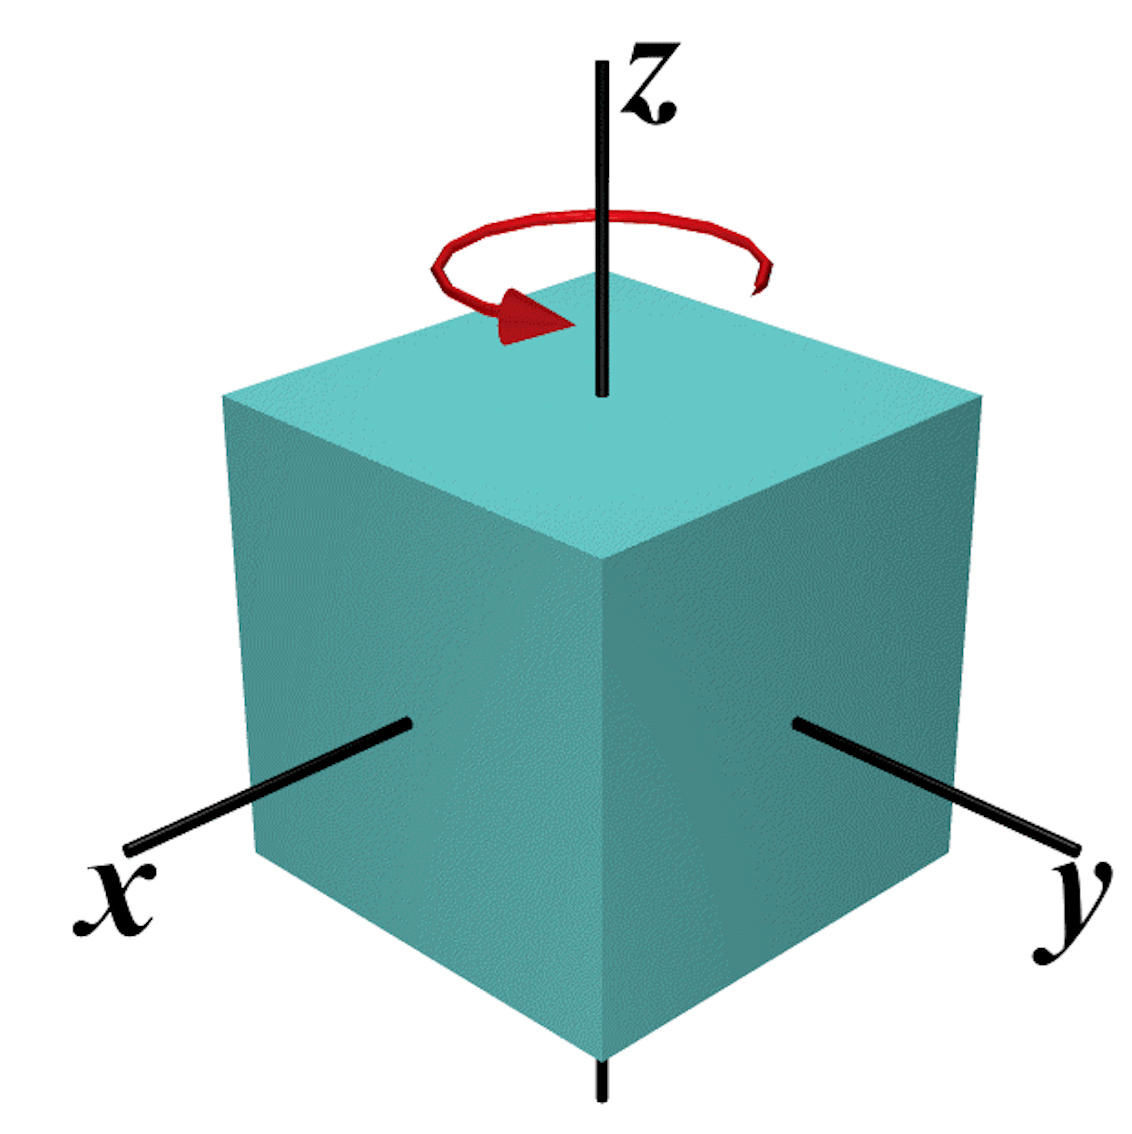
\includegraphics[width=2in]{images/AxesOfCube.png}
\caption{Cube with 3 axes of rotation that give symmetries.}\label{fig:CubeRot}
\end{center}
\end{figure}


\begin {exercise}{Cube1}
\begin {enumerate}[(a)]
\item Give rotations that take the bottom face ($z_-$ ) to each of the faces $x_-,x_+,y_-,y_+$.
%$r_y$ or $r_y^{-3}$takes $z_-\rightarrow x_-$, $r_y\compose r_z^2$ or  $r_y^{-1}$ or $r_y^3$ takes $z_-\rightarrow x_+$, $r_x^3$ or $r_x^{-1}$takes $Z_-\rightarrow y_-$, r_x$ or $r_x^{-3}$takes $z_-\rightarrow y_+$,
\item Give rotations that take the face $y_- $ to each of the faces $x_-,x_+,y_+,z_-,z_+$.
%$r_z^{-1}$or $r_x^{3}$ takes $y_-\rightarrow x_-$, $r_z$ or $r_z^{-3}$ takes %$y_-\rightarrow x_+$, $r_z^{-2}$ or $r_z^{2}$takes $y_-\rightarrow y_+$, $r_x$ %or r_x^{-3} takes $y_-\rightarrow z_-$, $r_x^{-1}$or $r_x^{3}$ takes $y_-\rightarrow z_+$,
\item Let's define a notation for the cube's vertices as follows.  For example, $+++$ represents the vertex in the first octant ($x>0,y>0,z>0$).  The vertex $+-\,-$ will be in the octant where $x>0,y<0,z<0$ (Which is the vertex at lower left in Figure~\ref{fig:CubeRot}).  Give rotations that take the vertex $+-\,-$ to each of the of the vertices 
\[ +++, ~-\,++,~+\,-\,+,~ ++\,-,~-\,-\,+,~-\,+\,-,~-\,-\,-. \]
%$r_x^2$or $r_x^{-2}$ takes $+-\,-\rightarrow +++$,
 %$r_x$ or$r_x^{-3}$ takes $+-\,-\rightarrow -\,++$, 
%$r_x\compose r_y^2$ takes $+-\,-\rightarrow -\,++$, 

\item Let's denote the edges of the cube as follows.  For example, $\overline{x_+z_-}$ represents the edge where the faces $x_+$ and $z_-$ meet.  The edge $\overline{x_+y_-}$ is where the faces $x_+$ and $y_-$ meet.  (This is the left, front-facing edge of cube in Figure~\ref{fig:CubeRot}.)  
\begin {enumerate}[(i)]
\item Using the above notation, list all edges of the cube.
\item Give rotations that take the edge $\overline{x_+y_+}$ to each of the other edges. 
\end {enumerate}
\end{enumerate}
\end{exercise} 
%$\overline{x_+y_-}$, $\overline{x_+z_+}$,$\overline{x_+z_-}$,$\overline{x_-%y_+}$,$\overline{x_-y_-}$,$\overline{x_-z_+}$,$\overline{x_-z_-%}$,$\overline{y_+z_+}$,$\overline{y_+z_-}$,$\overline{y_-z_+}$,$\overline{y_-z_-}$,
%In part (a) of the previous exercise, we saw that we could rotate the bottom face of the cube ($z_-$) to any other face.  We can use this information to rotate between any two faces.  For example, if we want to rotate the top face ($z_+$) to $x_+$, we can do this in two stages as follows.  First, we can rotate $z_+$ to $z_-$ using $r_x^{-1}\compose r_x^{-1}$ (which is the \emph{inverse} of the rotation that we used to take $z_-$ to $z_+$).  Second, we follow this by a rotation that takes $z_-$ to $x_+$ (such as $r_y^{-1}$).  In summary, we then have that 
From the previous exercise it's pretty clear that for any two faces of a cube there is at least one symmetry that takes the first face to the second.  In other words, if $A$ and $B$ represent faces then there always exists a symmetry $g$ such that $gA=B$.  This example motivates the following definition.

\begin{defn}\label{GEquivalent}
If a group $G$ acts on a set $X$ and $x, y \in X$, then $x$ is said to be
\bfii{ $G$-equivalent\/}\index{$G$-equivalent} to $y$ if there exists a
$g \in G$ such that $gx =y$. We write $x \sim_Gy$ or $x \sim y$ if
two elements are $G$-equivalent.
\end{defn}
By this definition we can say that all faces of a cube are $G$-equivalent to each other under the group of rotational symmetries of a cube.
The notation we're using strongly suggests that $\sim_G$ must be an equivalence relation.  If fact this is true:

\begin{thm}
Let $X$ be a $G$-set. Then $G$-equivalence is an equivalence relation
on $X$. 
\end{thm}
\begin{proof}
The relation $\sim$ is reflexive since $ex = x$. Suppose that $x \sim
y$ for $x, y \in X$. Then there exists a $g$ such that $gx = y$. In
this case $g^{-1}y=x$; hence, $y \sim x$. To show that the relation is
transitive, suppose that $x \sim y$ and $y \sim z$. Then, there must
exist group elements $g$ and $h$ such that $gx = y$ and $hy= z$. So $z
= hy = (hg)x$, and $x$ is equivalent to $z$.
\end{proof}

Recall from Chapter~\ref{EquivalenceRelationsChap} that every equivalence relation on a set $X$ is associated with a partition of $X$, where a partition is a collection of disjoint subsets whose union is $X$. Each set in this partition is called an \bfii{equivalence class}.\index{Equivalence class}

\begin {exercise}{Cube2}
Consider the edge $\overline{y_+z_+}$ of a cube.  What is the equivalence class of this edge under $G$-equivalence, where $G$ is the groups of rotational symmetries of a cube?
\end {exercise}

In the case of a cube where $X=\{\text{faces}\}\cup\{\text{edges}\}\cup\{\text{vertices}\}$ The three sets $\{\text{faces}\},\{\text{edges}\},\{\text{vertices}\}$ are disjoint equivalence classes whose union is $X$. We call each of these sets an \emph{orbit} of $X$ under $G$.  In general, we have the following definition.

\begin{defn} \label{noteorbit}
If $X$ is a $G$-set, then each set in the partition of $X$ associated with
$G$-equivalence is called an\bfii{ orbit\/}\index{Orbit!Of a $G$-set} of $X$ under $G$. We will denote the orbit that contains an element $x$ of $X$ by
${\cal O}_x$. 
\end {defn}
The next example shows how these concepts apply to permutation groups as well.

\begin{example}{Orbit1}
Let $G$ be the permutation group defined by
\[
G =\{(1), (1 23), (1 3 2), (4 5), (1 2 3)(4 5), (1 3 2)(4 5) \}
\]
and $X = \{ 1, 2, 3, 4, 5\}$. Then $X$ is a $G$-set. There are permutations in $G$ that take $1\rightarrow2$, $1\rightarrow3$, $2\rightarrow3$, and vice versa. There are also permutations that take $4\rightarrow 5$ and vice versa.  So the orbits are $\{1, 2, 3\}$ and $\{4, 5\}$. 
\end{example} 
 
\begin{exercise}{orbits2}
\begin{enumerate}[(a)]
\item Let $G=\{\var{id},\mu_1\}$ which is a subgroup of $S_3$ (the symmetry group of an equilateral triangle) (See Figure~\ref{groups_s3_symmetry_fig} in Section~\ref{SymmetryGroup}.) Let $X=\{A,B,C\}$ be the set of vertices of an equilateral triangle. List the orbits of $X$ under $G$
\item Let $G$ be the permutation group defined by
\begin{align*}
G =&\{(1), (1358),(1538), (1853), (247),(274), (1358)(247),(1538)(247),\\
&~~ (1853)(247),(1358)(274),(1538)(274),(1853)(274) \}
\end{align*}
and $X = \{ 1, 2, 3, 4, 5,6,7,8\}$. Then $X$ is a $G$-set.  List the orbits of $X$ under $G$.
\end{enumerate}
\end {exercise}


\subsection{Stabilizers, stabilizer subgroups, and fixed point sets}

 Let's return to the cube to illustrate another new concept. Every rotation of a cube has an axis of rotation as well as an angle.   
 For rotations which are symmetries we've considered 3 possible axes, passing through opposite pairs of faces. 
For every pair of opposite faces, all rotational symmetries whose axis passes through those faces leaves them fixed.   Note that these rotations form a subgroup.  Similar subgroups are obtained when we take the axes through opposite edges, or opposite vertices. These are all examples of \emph{stabilizer subgroups}. The general definition is as follows.

\begin {defn}\label {StabilizerSubgroups} 
Given that $X$ is a $G$-set and  $x \in X$, let $G_x$ be the set of  group elements $g$ that fix $x$:  in other words, $gx=x$.  Then $G_x$ is called the \bfii{ stabilizer subgroup}\index{Subgroup!stabilizer} or \bfii{ isotropy 
subgroup}\index{Subgroup!isotropy} of $x$.
\end{defn}

\begin {exercise}{Stabilizer1}
Given any $x$ in $X$, prove that the stabilizer subgroup $G_x$  is a subgroup of $G$.  (Recall this involves proving closure under composition and inverse.)
\end {exercise}

On the other hand, each element of $G$ has an associated subset of $X$ that it leaves unchanged. 
Recall that the group of rotations of a cube act on the set:   $X=\{\text{faces}\}\cup\{\text{edges}\}\cup\{\text{vertices}\}$.  Any rotation about the $x$ axis ($r_x^n$) leaves the faces $x_+$ and $x_-$ fixed.   $\{x_+,x_-\}$is a subset of $X$. Similarly, $\{y_+$ ,$y_-\}$ and $\{z_+,z_-\}$ are  fixed by rotations about the $y$ axis and $z$ axis, respectively.   Thus, $\{x_+,x_-\},\{y_+,y_-\},\{z_+,z_-\},$  are all examples of \emph{fixed point sets} in $X$.
This leads to another definition:

\begin{defn} \label {FixedPoint}
Let $G$ be a group acting on a set $X$, and let $g$ be
an element of $G$. The \bfii{ fixed point set}\index{Fixed point
set!of a group element} of $g$ in $X$, denoted by $X_g$, is the set of 
all $x \in X$ such that $gx = x$.
\end{defn}
\noindent
It is important to remember that $X_g \subset X$ and $G_x \subset G$. 

Let's use this notation to describe some stabilizer subgroups and fixed point sets for familiar examples of group actions.

\begin {example}{FixedPoint1}
Let $G$ be the rotational symmetries of a cube and $X=\{\text{faces}\}\cup\{\text{edges}\}\cup\{\text{vertices}\}$
The fixed point set of $\var{id}$ is: 

$$X_{\var{id}}=\{\text{faces}\}\cup\{\text{edges}\}\cup\{\text{vertices}\}$$
since the identity rotation  leaves the entire cube unchanged.  
\end {example}

\begin {example}{FixedPoint2}
Let's consider the stabilizer subgroups for the faces of a cube.  These contain the elements of the group $G$ of rotations of the cube that leave each face unchanged.  The stabilizer subgroups for the faces are:
$$\begin {array} {c}
G_{x_+}=G_{x_-}=\{\var{id},r_x,r_x^2,r_x^3\}\\
G_{y_+}=G_{y_-}=\{\var{id},r_y,r_y^2,r_y^3\}\\
G_{z_+}=G_{z_-}=\{\var{id},r_x,r_x^2,r_x^3\}
\end {array}$$
\end{example}

\begin{example}{FixedPoint3}
Let $X = \{1, 2, 3, 4, 5, 6\}$ and suppose that $G$ is the permutation
group given by the permutations 
$$\{(1), (1 2)(3 4 5 6), (3 5)(4 6), (1 2)( 3 6 5 4)\}.$$
Then the fixed point sets of $X$ under the action of $G$ for the different group elements are
$$
\begin{array}{c}
X_{(1)} = X, \\
X_{(3 5)(4 6)} = \{1,2\}, \\
X_{(1 2)(3 4 5 6)} = X_{(1 2)(3 6 5 4)} = \emptyset,
\end{array}
$$
and the stabilizer subgroups for the different elements of $X$ are
$$
\begin{array}{c}
G_1 = G_2 = \{(1), (3 5)(4 6) \}, \\
G_3 = G_4 = G_5 = G_6 = \{(1)\}.
\end{array}
$$
\end{example}

%\begin{thm}
%Let $G$ be a group acting on a set $X$ and $x \in X$. The stabilizer
%group, $G_x$, of $x$ is a subgroup of $G$. 
%\end{thm}
%\begin{proof}
%Clearly, $e \in G_x$ since the identity fixes every element in the
%set $X$. Let $g, h \in G_x$. Then $gx = x$ and $hx = x$. So $(gh)x =
%g(hx) = gx = x$; hence, the product of two elements in $G_x$ is also
%in $G_x$. Finally, if $g \in G_x$, then $x = ex = (g^{-1}g)x =
%(g^{-1})gx = g^{-1} x$. So $g^{-1}$ is in $G_x$. 
%\end{proof}

\begin{exercise}{}
Let $G = S_4$ (the permutations of 4 elements), and let $X = \{1,2,3,4\}$.  $X$ is a $G$-set.
\begin{enumerate}[(a)]
\item
Give $G_2$, $G_4$, and $G_2 \cap G_4$.  Is $G_2 \cap G_4$ a group? \emph{Explain} your answer.
\item
Give $X_{(123)}$, $X_{(234)}$,and  $X_{(123)} \cap X_{(234)}$.
\item
Repeat part (a) with $G=A_4$ (the group of even permutations on 4 elements).
\item
Repeat part (b) with $G=A_4$ (the group of even permutations on 4 elements).
\end{enumerate}
\end{exercise} 
As usual, we will denote the number of elements in the fixed point set of an
element $g \in G$ by $|X_g|$, the number of elements of the stabilizer subgroup of $x\in X$ as $|G_x|$ and the number of elements in the orbit of $x \in X$ by $|{\cal O}_x|$.

\begin{exercise}{}
Let $G = S_n$ (the permutations of n elements), and let $X = \{1,2,\ldots n \}$.  $X$ is a $G$-set.
\begin{enumerate}[(a)]
\item
What is $|G_1|$? What is $|G_2|$? What is $|G_k|$ where $k \in X$?  (Recall that $|S_n| = n!$)
\item
If $g$ is a $3$-cycle, then what is $|X_g|$? What if $g$  is a 5-cycle?  (You may assume that $n \ge 5$).
\item
Give a general formula for $X_g$, where $g$ is a $k$-cycle ($2 \le k \le n$).
\item
Repeat part (a) with $G = A_n$ (the even permutations of $n$ elements).
\item
Repeat part (b) with $G = A_n$.
\item
Repeat part (c) with $G = A_n$.
\end{enumerate}
\end{exercise}

%Recall from Chapter\ref{cosets} that the \emph{index} of $G_x$ in $G$ (denoted by $[G:G_x]$) is the number of cosets of $G_x$. 

\subsection{Counting formula for the order of  polyhedral rotational symmetry groups}

It is possible to characterize the size of the rotational symmetry group $G$ for a regular polyhedron in terms of $|{\cal O}_x|$and $|G_x|$ . We'll show this with an example.

\begin{example}{CountingFormula1} 
Consider our old friend the group of rotational symmetries of a cube acting on $X=\{\text{faces}\}\cup\{\text{edges}\}\cup\{\text{vertices}\}$. We've seen that $G_{x_+}=\{\var{id},r_x,r_x^2,r_x^3\}$ is the stabilizer subgroup for $x_+$.  Thus there are four rotations that take $x_+$ to itself.  We've also seen that there's at least one rotation that takes $x_+$ to each of the six faces of the cube:  this is the same thing as saying that the orbit of a face is the set of all faces.  Each of these rotations can be composed with any of the elements of $G_{x_+}$ for a total of $6\cdot 4=24$ rotational symmetries of a cube.  To summarize, we've discovered that 
$$|G|=|G_{x_+}|\cdot |{\cal O}_{x_+}|.$$
Note that $x_+$ was an arbitrary choice: we could use this argument with any of the faces and obtain the same result.
\end{example}

In the previous example we used faces to count the rotational symmetries of a cube but we could use edges or vertices as well.  In the next exercise we'll consider edges and in the following one we'll consider vertices.   A model of a cube might help with these exercises (see Figure~\ref{fig:CubeFold}).

\begin{figure}[ht]
\begin{center}
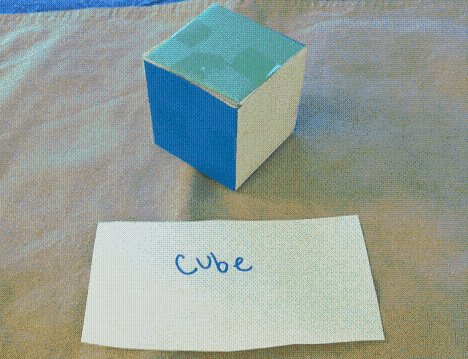
\includegraphics[width=2.5in]{images/CubeFold.png}
\caption{A paper cube to print, cut and fold from www.korthalsaltes.com}
 \label{fig:CubeFold}
\end{center}
\end{figure}

\begin {exercise}{CountingFormula2}
\begin {enumerate}[(a)]
\item Find the stabilizer subgroup for the edge $\overline{x_+,z_+}$. 
\hyperref[sec:actions:hints]{(*Hint*)}
%$G_{\overline{x_+,z_+}}=\{r_x^2\compose r_y, \var{id}\}$
\item Find the stabilizer subgroup for the edge $\overline{x_-,y_+}$.
% $G_{\overline{x_-,y_+}}=\{r_y^2\compose r_z^{-1}, \var{id}\}$
\item In Example ~\ref {example:actions:CountingFormula1} we constructed a formula for $|G|$ in terms of $| G_{x_+}|$ and $|{\cal O}_{x_+}|$.  Can you do the same thing with $\overline{x_+,z_+}$ using part (a)?  Can you do the same thing with $\overline{x_-,y_+}$ using part (b)?  
\item Find the stabilizer subgroup for the vertex $+,+,+$ 
\hyperref[sec:actions:hints]{(*Hint*)}
% $G_{+,+,+}=\{var{id}, r_y\compose r_z, r_z^{-1}\compose r_y^{-1} \}$
\item Find the stabilizer subgroup for the vertex $+\,,-\,,+$. 
%$G_{+\,-\,+}=\{var{id}, r_y\compose r_z^{-1}, r_z\compose r_y^{-1} \}$
\item Using parts (d) and (e), construct alternative formulas for $|G|$.
\end{enumerate}
\end{exercise}

From the previous example and exercises, it seems we have a general formula:  if $G$ acts on $X$ and $x\in X$, then 
$$|G|=|G_x|\cdot|{\cal O}_x|.$$

This may remind you of \emph{Lagrange's Theorem}, which we proved in %/Proposition~\ref{LagrangeTheorem} in section ~\ref{sec:LagThm} of Chapter ~\ref{cosets}:  
$$|G|=|H|\cdot [G:H], $$
where $H$ is any subgroup of $G$.  If we replace $H$ with $G_x$, this becomes $$|G|=|G_x|\cdot [G:G_x]. $$
Comparing with our previous formula, we get
 $$|{\cal O}_x|=[G:G_x].$$
Let's give a real mathematical proof of this.

\begin{thm}\label{prop:CountingFormula}(\emph{Counting formula}):~~
Let $G$ be a group and $X$ a $G$-set. If $x\in X$,
then $|{\cal O}_x| = [G:G_x]$. 
\end{thm}

\begin{proof}
In general, a good way to show that two sets are the same size is to show that there is a \emph{bijection}. (1-1 and onto map) between the two sets.  
 We will define a map $\phi$
between the orbit ${\cal O}_x$ and the set of left cosets of $G_x$ in $G$ as follows. Let $y \in {\cal O}_x$. Then there 
exists a $g$ in $G$ such that $g x = y$. Define $\phi$ by $\phi( y ) 
= g G_x$. Note that this coset contain an element $ge=g$:  so it contains an element that takes $x\rightarrow y$.  

Before we can show that $\phi$ is a bijection, we must first show that $\phi(y)$ is well-defined for any $y$, and does 
not depend on our selection of $g$. Suppose that $g'$ is another 
element in $G$ such that $g'x = y$. Then $g x = g' x$ or $x= g^{-1} g' x$. 
By the definition of the stabilizer subgroup $G_x$, $g^{-1}g'\in G_x$. By Proposition~\ref{cosets_theorem_1} in Section \ref{sec:CosetsPartitions}, it follows that 
 $g G_x = g' G_x$. Thus, $y$ gets mapped to the same 
coset regardless of the choice of group element.


To show that $\phi$ is one-to-one, we'll assume that $\phi(x_1) =
\phi(x_2)$, and show that this means that $x_1=x_2$. Here we go: 

Recall that $\phi(x_1)$ is defined as a coset of $G_x$ that contains an element $g_1$ that satisfies $g_1x=x_1.$   Similarly,  $\phi(x_2)$ , contains  an element $g_2$ that satisfies $g_2x=x_2$. But we're assuming that $\phi(x_1) =
\phi(x_2)$.  This means that $g_1$ and $g_2$ are in the same coset of $G_x$.  

Now consider the expression $g_1(g_1^{-1}g_2)x$. On the one hand, by the associative law we get:
$$(g_1g_1^{-1})g_2x=g_2x=x_2.$$ 
 On the other hand, by Proposition~\ref{cosets_theorem_1} in the Cosets chapter, it follows that $g_1^{-1}g_2$ is in $G_x$, so that $g_1^{-1}g_2x=x$.  This means that we also have:
$$g_1(g_1^{-1}g_2)x=g_1x=x_1.$$
  Therefore $x_1=x_2$.  This completes the proof that $\phi$ is 1-1.

Finally, we must show
that the map $\phi$ is onto: that is, every coset of $G_x$ is in the range of $\phi$. This is much quicker than the proof of 1-1. 
Let $g G_x$ be any  left coset. If $g x =y$, then $\phi(y) = g G_x$.  Thus $gG_x$ is in the range of $\phi$, and the proof is finished.
\end{proof}

\subsection{Representing $G$ in terms of stabilizer subgroups}
We can approach the structure of the group of rotational symmetries of a cube from another direction.  We've talked about stabilizer subgroups, and we can see how these subgroups ``fit together'' within $G$.
For example, we've seen that for every face there are three rotations (besides the identity) that leaves that face fixed. These rotations correspond to 90, 180, and 270 degree rotations of a square: so they have order 4,2, and 4 respectively.\footnote{Recall that the ``order'' of a group element $g$ is the smallest positive integer $n$ such that $g^n = \var{id}$.} So for each face, there are two rotations of order 4 and one rotation of order 2 in the stabilizer of that face. Since there are 6 faces of a cube, this seems to imply that there must be twelve rotations of order 4 and six rotations of order 2 associated with the stabilizers of the different faces.  Unfortunately, this is not quite true. The reason is that any rotation that leaves the front face fixed also leaves the back face fixed. So the stabilizer of the front face is the same as the stabilizer  of the back face. In fact, the faces of the cube are stabilized in pairs: front-back, left-right, and top-bottom. Since there are 3 pairs, this means that we only have 6 rotations of order 4 and 3 rotations of order 2. If we add in the identity, this gives a total of 10 rotations. But we've already shown that the group of rotational symmetries of a cube has 24 elements. Where are the other 14?
Well, we haven't exhausted the possible stabilizers. Consider for instance the stabilizer of a vertex. We know that 3 faces meet at each vertex. So if I twirl the cube around the vertex, the three faces can rotate into each other. So besides the identity, there are two rotations of order 3. As with the faces, each vertex has a corresponding opposite vertex--so the vertices are stabilized in pairs. Since there are 8 vertices, this means there are 4 pairs, which means there are 8 rotations of order 3. This brings us up to a total of 18 rotations. Where are the other six?

\begin{exercise}{Stabilizers1}
Consider the edges of a cube.
\begin{enumerate}[(a)]
\item
For each edge, how many rotations (besides the identity) leave that edge fixed?
% Two faces meet at each edge so beside the identity 1 rotation that leaves each edge fixed.  
\item
What are the orders of the rotations that leave an edge fixed?
%order 2 
\item
Do edges come in pairs or not?  If so give the pairs, if not, explain why not.
% edges come in pairs a rotation that stabilizes $\overline{x_+,z__+}$ will also stabilize $\overline{x_-,z_-}$ and $\overline{y_-,z_+}$ is stabilized by the same rotation as $\overline{y_+,z_-}$
\item
How many additional group elements do we obtain from the stabilizers of the different edges, and what are their orders? 
% There are 6 pairs of edges each stabilized by one element of order two as well as the identity.  There are 6 group elements in the stabilizers of the different edges.
\end{enumerate}
\end{exercise}
\begin{exercise}{Stabilizers2}
Complete the following table to characterize the group elements of the rotational symmetries of a cube.
\footnote{We refer the reader once more to the video: \url{www.youtube.com/watch?v=gBg4-lJ19Gg}).}

\begin{tabular}{| l |c|c| r |}\hline
  Number of elements & order of the element & Type of set that it stabilizes \\ \hline
  1 & 1 & entire cube (identity) \\ \hline
  2 & 4 & face \\ \hline
 -- & -- & -- \\ \hline
-- & -- & -- \\ \hline
-- & -- & -- \\ \hline
\end{tabular}
\end{exercise}
%\begin{tabular}{ |l |c|c| r |}\hline
%  Number of elements & order of the element & Type of set that it stabilizes \\ \hline
%  1 & 1 & entire cube (identity) \\ \hline
%  6 & 4 & face \\ \hline
% 3 & 2 & face \\ \hline
%8 & 3& vertex \\ \hline
%6& 2 & edge \\ \hline
%\end{tabular}
\section{Examples of other regular polyhedral rotation groups}
Let's get to know some other regular polyhedra using orbits and stabilizer subgroups to describe their rotational symmetry groups.
\subsection{The tetrahedron}
Consider a regular tetrahedron, as shown in Figure~\ref {fig:TetRot} This polyhedron has 4 faces, 6 edges and 4 vertices.  Each face is a triangle and each face is opposite a vertex. We will consider the rotations of a tetrahedron around 4 axes.  Each axis passes through a vertex and the face opposite that vertex. See Figure~\ref {fig:TetRot}. For example, a rotation of the axis through vertex $A$ will also stabilize face $a$.  We can call this axis $\overset{\leftrightarrow}{Aa}$.  Similarly, we will call the other axes $\overset{\leftrightarrow}{Bb}$, $\overset{\leftrightarrow}{Cc}$ and $\overset{\leftrightarrow}{Dd}$.

\begin{figure}[ht]
\begin{center}
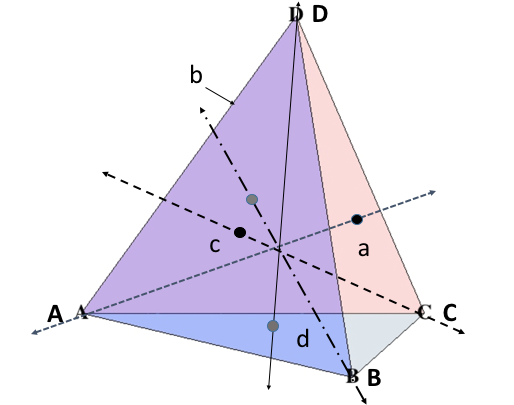
\includegraphics[width=2.5in]{images/TetrahedronC.png}
\caption{Tetrahedron with 4 axes of rotation that give symmetries. Figure modified  from - https://inspirehep.net}\label{fig:TetRot}
\end{center}
\end{figure}


Note that each of these axes rotates a triangular face. We'll write one counterclockwise rotation of face $a$ around $\overset{\leftrightarrow}{Aa}$ as $r_{Aa}$ (and similarly for the other axes).
An animation of the rotations of a tetrahedron is available at:

\url{https://www.youtube.com/watch?v=qAR8BFMS3Bc}

You can also make your own tetrahedron like the one in Figure~\ref{fig:TetraFold}.

\begin{figure}[ht]
\begin{center}
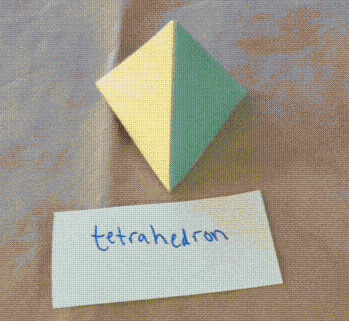
\includegraphics[width=2.5in]{images/TetrahedronFold.png}
\caption{Tetrahedron to print, cut and fold from www.korthalsaltes.com}
 \label{fig:TetraFold}
\end{center}
\end{figure}

\begin{exercise}{Tetra 1}
\begin{enumerate}[(a)]
\item How many degrees does $ r_{Aa}$ rotate face $a$?
% 120 degrees
\item What is the order of $r_{Aa}$?
% order 3
\end{enumerate}

\end{exercise}
Consider the tetrahedron in Figure~\ref{fig:TetRot}.  The rotation $r_{Cc}$ takes vertex $D$ to vertex $A$ and face $d$ to face $a$.  

\begin {exercise}{tetra2}
We'll find it useful later to represent these rotations as permutations.
\begin {enumerate}[(a)] 
\item Represent each of the rotations $r_{Aa},$ $r_{Bb},$ $r_{Cc},$ $r_{Dd}$ as permutations on the set of vertices.
\item Represent each of the rotations $r_{Aa}$$r_{Bb}$$r_{Cc}$$r_{Dd}$ as permutations on the set of faces.
\end{enumerate}
\end {exercise}
\begin {exercise}{Tetra3}
\begin {enumerate}[(a)]
\item Give rotations that takes face $c$ to each to each of the other faces $a, b, d$.
\item Give rotations that takes vertex $D$ to each of the other vertices.
\item Consider the edges of the tetrahedron.  Denote the edge between the vertices $C$ and $D$ as $\overline{CD}$: and other edges similarly.  Use this notation to name each of the edges of the tetrahedron.
 \item Give a rotation that takes edge $\overline{CD}$ to each of the other edges.
\end{enumerate}
\end{exercise} 
\begin {exercise}{Tetra4}
Consider the vertex $A$ of a tetrahedron.  What is the equivalence class of this vertex under $G$-equivalence, where $G$ is the groups of rotational symmetries of a tetrahedron?   (Note:  This $G$-equivalence class is the same as orbit of $A$. which we denote as ${\cal O}_A$.)
\end {exercise}

%$ cal{O}_A =\{A,B,C,D\}

Just as with the cube, the rotation group $G$ of any polyhedron acts on the set $X=\{\text{faces}\}\cup\{\text{edges}\}\cup\{\text{vertices}\}$. Recall that each group element $g\in G$ has a \emph{fixed point set} $X_g\in X$ that it leaves unchanged: that is, $gx=x$ for any $x\in X_g$. Let's find some fixed point sets for rotations of the tetrahedron.

\begin {exercise}{Tetra5}
\begin {enumerate}[(a)]
\item Let $G$ be the rotational symmetries of a tetrahedron what is the fixed point set of $r_{Bb}$
%$X_{r_{Bb}}=\{B,b\}
\item What is the fixed point set of $r_{Bb}\compose r_{Dd}$? 
\hyperref[sec:actions:hints]{(*Hint*)}
%$X_{ r_{Bb}\compose r_{Db }}=\{A,a\}$
\item What is the fixed point set of $r_{Bb}^{-1}\compose r_{Dd}$?
\item Give all rotations that fix the set $\{D,d\}$. 
%\item Give a rotation that fixes the following set}{\overline{AB},\overline{CD}\}
\end{enumerate}
\end {exercise}

Let's consider the stabilizer subgroups for the faces and vertices of a tetrahedron. \emph {hint} $R_{Bb}^2$ is the 240 degree rotation around the axis $\overset{\leftrightarrow}{Bb}$, it will stabilize face $b$.  

\begin{exercise}{Tetra5a}
Find the stabilizer subgroups for each of the following:
$G_{A}, G_{B}, G_{C}, G_{D}$, $G_{a}, G_{b}, G_{c}, G_{d}$. Which subgroups are equal?
\end{exercise}

Let's use the stabilizer subgroups above to determine the total number of rotational symmetries of a tetrahedron.  

\begin{exercise}{Tetra6} 
Let $G$ be the rotational symmetries of a tetrahedron.  As in Example~\ref{example:actions:CountingFormula1} construct a formula for $|G|$ in terms of $| G_{A}|$ and $|{\cal O}_{A}|$.  \end {exercise}
So far we've found 4 rotational axes and two rotations around each axis (besides the identity). This gives nine rotations.  As we can see there must be more rotational symmetries of a tetrahedron than we've discovered so far.  Let's try to find them. 

\begin {exercise}{Tetra7}
\begin {enumerate}[(a)]
\item Find the stabilizer subgroup for the edge $\overline{CD}$. 
\item Find the stabilizer subgroup for the edge $\overline{AB}$.
\item How many different group elements (besides the identity) stabilize at least one edge?
\item Are there any group elements that are not stabilizers of either an edge or a face?  Explain your answer.
\end{enumerate}
\end{exercise}	

\begin {exercise}{Tetra8}
In Exercise~\ref{exercise:actions:Tetra6} we constructed a formula for $|G|$ in terms of$| G_{A}|$ and $|{\cal O}_{A}|$.  Can you do the same thing using $| G_{\overline{AB}}|$ and $|{\cal O}_{\overline{AB}}|$?
\end{exercise}

\begin{exercise}{Tetra9}
Complete the following table to characterize the group elements of the rotational symmetries of a tetrahedron.  We show two rows, how many more to complete the table?
  
\begin{tabular}{| l |c|c| r |} \hline
  Number of elements & order of the element & Type of set that it stabilizes \\ \hline
  --&  --& entire tetrahedron (identity) \\ \hline
  -- & --& face and vertex \\  
\end{tabular}
\end{exercise}
% begin{tabular}{ l c r }
  %Number of elements & order of the element & Type of set that it stabilizes \\
% 1 & 1 & entire tetrahedron (identity) \\
  %8 & 3 & face and vertex \\
 % 3 & 2 & edge \\
%\end{tabular}
\subsection{The octahedron}
Another regular polyhedron is the octahedron.  We will see that in some ways an octahedron is like a cube. 
When viewed on a vertical $z$ axis the octahedron has no vertical or horizontal faces.  See Figure~\ref{fig:OctaRot}.  We can call a 90 degree counterclockwise rotation around the vertical axis $r_z$ (and similarly for rotations around the $x$, and $y$ axes).
Since each vertex of the octahedron lies on an axis, we can use the $x,y$, and $z$ axis to label the vertices.  For example $y_+$ is the vertex on the positive $y$ axis.   We can also name the edges using this notation for their endpoints.   Let's use the axes to label the faces of the octahedron too.  Consider Figure~\ref{fig:OctaRot}, we'll refer to the the face in the first octant as $\triangle_{ +++}$ (the other faces will be labeled similarly).

\begin{figure}[ht]
\begin{center}
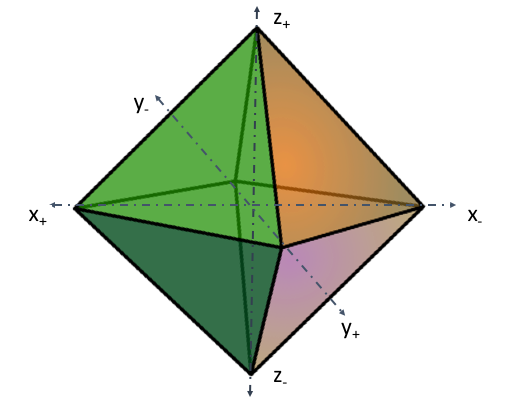
\includegraphics[width=2.5in]{images/AxesOfOctahedron.png}
\caption{Octahedron with 3 axes of rotation that give symmetries. Figure modified from https://en.wikipedia.org/wiki/File:Octahedron.svg
}\label{fig:OctaRot}
\end{center}
\end{figure}


\begin {exercise}{Octa1}
\begin {enumerate}[(a)]
\item List all the faces of the octahedron using the notation above.
\item Based on Figure~\ref{fig:OctaRot}  how many faces does an octahedron have? How many vertices?  How many edges?
\end{enumerate}
%8 faces, 12 edges, 6 vertices
\end {exercise}

A model of an octahedron might help with the following exercises.  You can make one like the one in Figure~\ref{fig:OctaFold}.

\begin{figure}[ht]
\begin{center}
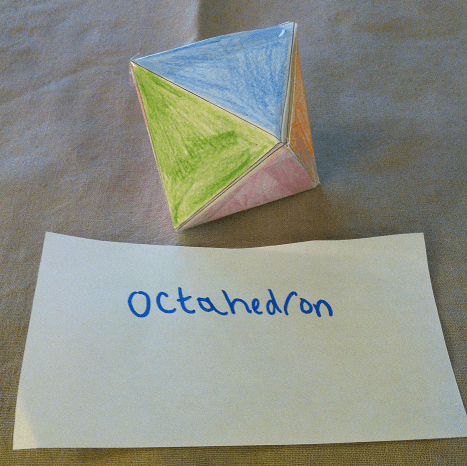
\includegraphics[width=2.5in]{images/OctahedronFold.png}
\caption{A paper octahedron to print, cut and fold (from \url{www.korthalsaltes.com}).}
 \label{fig:OctaFold}
\end{center}
\end{figure}

\begin{exercise}{Octa2}
What is the order of $r_z$?
%$|r_z|=3$
\end{exercise}

\begin{exercise}{Octa3}
\begin {enumerate}[(a)]
\item Give rotations that take $\triangle _{+++}$ to each to each of the other faces.
\item Give rotations that take  $x_-$ to each of the other vertices.
\item Give a rotation that takes edge $\overline{z_+y_+}$ to each of the other edges.
\end{enumerate}
\end{exercise} 
\begin {exercise}{Octa4}
Consider the edge $\overline{x_-y_+}$ of a octahedron. What is ${\cal O}_{\overline{x_-y_+}}$?
\end {exercise}

\begin {exercise}{Octa5}
\begin {enumerate}[(a)]
\item Let $G$ be the rotational symmetries of an octahedron what is the fixed point set of $r_{y}\compose r_{z}$?
%$X_{r_{y}\compose r_{z}}=\{x_+,x_-\}$
\item What is the fixed point set of $r_{y}^2\compose r_{x}$? 
%$X_r_{y}^2\compose r_{x}=\{\overline {y_+z_+},\overline{y_-z_-}\}$
\item What is the fixed point set of $r_{x}^2\compose r_{y}$?
\end{enumerate}
\end {exercise}

Let's consider the stabilizer subgroups for the faces and vertices of an octahedron.  
 
\begin{exercise}{Octa5a}
Find the stabilizer subgroups for each of the vertices of the octahedron. 
\hyperref[sec:actions:hints]{(*Hint*)}
\end{exercise}

Let's find the total number of rotational symmetries for the octahedron. 

\begin{exercise}{Octa6} 
Let $G$ be the rotational symmetries of an octahedron. Construct a formula for $|G|$ in terms of $| G_{y_+}|$ and $|{\cal O}_{y_+}|$ (see Example~\ref{example:actions:CountingFormula1}).
 \end {exercise}

So far we have discovered 10 rotational symmetries of an octahedron.  Three axis of 3 rotations each plus the identity.  By the previous exercise, there are still more to discover.  Here we go! 

\begin {exercise}{Octa7}
\begin {enumerate}[(a)]
\item Find the stabilizer subgroup for the edge $\overline{y_+~z_+}$. 
\item Find the stabilizer subgroup for the edge $\overline{y_-~z_-}$.
\item How many different group elements (besides the identity) stabilize at least one edge?
\end{enumerate}
\end{exercise}	

\begin{exercise}{Octa8}
\begin {enumerate}[(a)]
\item Find the stabilizer subgroup for the face $\triangle_{+ + +}$.
\item Find the stabilizer subgroup for the face $\triangle_{ -~-~-}$.
\item How many different group elements stabilize at least one face?
\end {enumerate}
\end{exercise}

\begin {exercise}{Octa9}
In Exercise ~\ref {exercise:actions:Octa6} we constructed a formula for $|G|$ in terms of $|G_{y_+}|$ and $|{\cal O}_{y_+}|$.  Can you do the same thing using $|G_{\triangle_{+ + +}}|$ and $|{\cal O}_{\triangle_{+ + +}}|$?
\end{exercise}

\begin{exercise}{Octa10}
Complete the following table to characterize the group elements of the rotational symmetries of an octahedron.  We show two rows, how many more to complete the table? 
 
\begin{tabular}{ |c| c | c |} \hline
  Number of elements & order of the element & Type of set that it stabilizes \\ \hline
  ---&  ---& entire  octahedron (identity) \\ \hline
  --- & ---&  vertices \\

\end{tabular}
\end{exercise}
% begin{tabular}{ l c r }
  %Number of elements & order of the element & Type of set that it stabilizes \\
% 1 & 1 & entire octahedron (identity) \\
  %8 & 3 & face  \\
 % 6 & 2 & edge \\
%6 & 4  & vertices\\
% 3 & 2 &  vertices\\
%\end{tabular}
\subsection{The dodecahedron}
Let's practice finding the elements of the rotation group of another regular polyhedron.  Consider the regular dodecahedron in Figure~\ref{fig:Dodeca}.  A dodecahedron has 12 faces and each face is a regular pentagon.  How many edges does this polyhedron have and how many vertices?  Well, since each of the twelve faces is a pentagon that seems to give $12\cdot 5=60$ edges.  But two faces meet at each edge, so we actually have $(12\cdot 5)/2=30$ edges.

\begin{figure}[ht]
\begin{center}
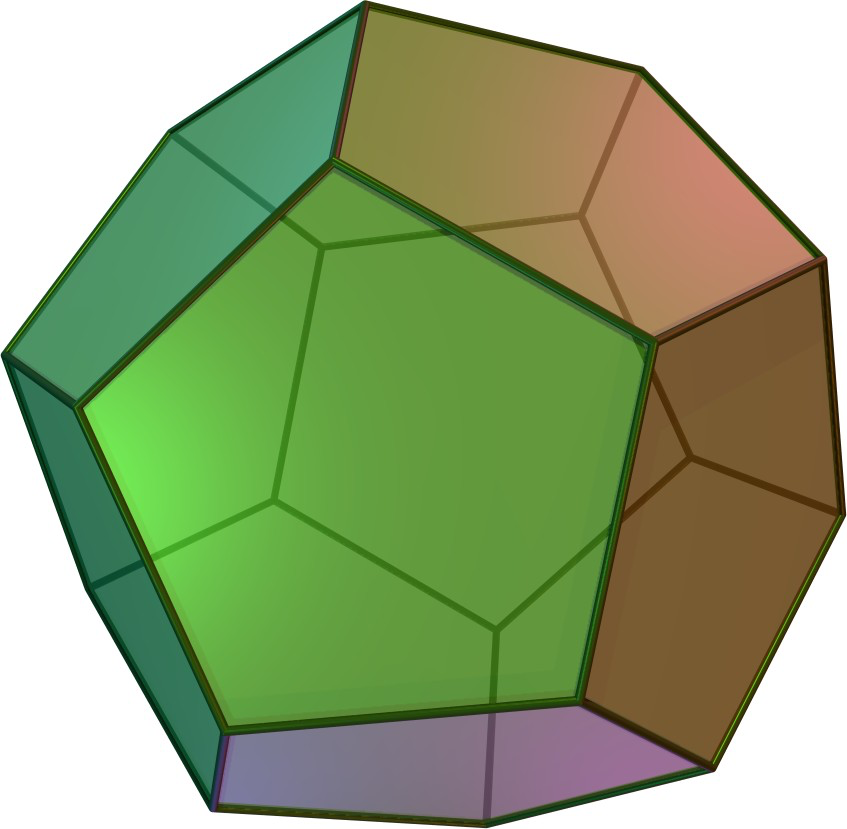
\includegraphics[width=2.5in]{images/Dodecahedron.png}
\caption{Dodecahedron. Source:\url{https://en.wikipedia.org}.}
\label{fig:Dodeca}
\end{center}
\end{figure}

You can also make your own dodecahedron to help you explore its rotational symmetries. See Figure~\ref{fig:DodecaFold}.

\begin{figure}[ht]
\begin{center}
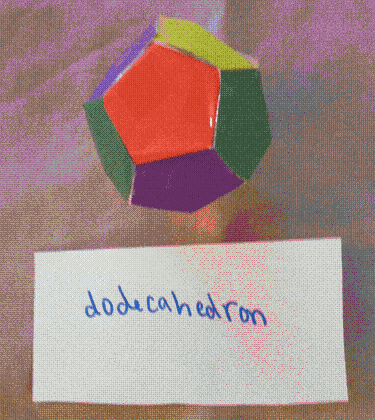
\includegraphics[width=2.5in]{images/DodecahedronFold.png}
\caption{A dodecahedron to print, cut and fold (from \url{www.korthalsaltes.com}).}
 \label{fig:DodecaFold}
\end{center}
\end{figure}

\begin{exercise}{Dodeca1}
Determine the number of vertices of a regular dodecahedron.
\end{exercise}
Let $f_1$ be one face of the dodecahedron.  An axis through the center of $f_1$ also passes the opposite face which is parallel to $f_1$. We'll call this opposite face $f_1^*$ and denote a counterclockwise rotation of $f_1$ about this axis as $r_{f_1}$.

\begin{exercise}{Dodeca2}
\begin {enumerate}[(a)]
\item What is the order of $r_{f_1}$?
% order 5
\item Let $G$ be the rotational symmetry group of a dodecahedron.  List all rotations in the stabilizer subgroup $G_{f_1}$.  What else do they stabilize?
%$G_{f_1}={\var{id},r_{f_1},r_{f_1}^2, r_{f_1}^3, r_{f_1}^4}$, $G_{f_1}$ will also stabilize the opposite (parallel) face.
\item What is $|G_{f_1}|?$
% $|G_{f_1}|=5$
\item How many group elements in $G$ stabilize at least 1 face?
%25 elements 4 rotations for each of 6 pairs of opposite faces, plus the identity.
\item What is $|{\cal O}_{f_1}|$?
%$|{\cal O}_{f_1}|=12$ The orbit of $f_1$ includes all faces of the dodecahedron.
\end{enumerate}
\end{exercise}
Now we can find the total number of rotational symmetries in $G$.

\begin {exercise}{Dodeca3}
Find $|G|$ in terms of $|G_{f_1}|$ and $|{\cal O}_{f_1}|$.
%$5\times 12=60$
\end {exercise}
So far we've found the number of the stabilizers of faces of the dodecahedron.  But, as with the cube and tetrahedron, we need axes of symmetry through edges and vertices as well.
Let $v_1$ be one vertex of the dodecahedron.  An axis of symmetry through $v_1$ will also pass through the opposite vertex, which we will call $v_1^*$.  A counterclockwise rotation about this axis is called $r_{v_1}$.

\begin{exercise}{Dodeca4}
\begin {enumerate} 
\item Find the order of $r_{v_1}$.
% order 3
\item List all rotations in the stabilizer subgroup $G_{v_1}$.  What else do they stabilize?
%$G_{v_1}={\var{id},r_{v_1},r_{v_1}^2}$ $G_{v_1}$ will also stabilize the opposite vertex.
\item How many group elements in $G$ (besides the identity) stabilize at least 1 vertex?
% 20 rotations 10 pairs of vertices, 2 rotations besides the identity stabilize each pair.
\item What is $|{\cal O}_{v_1}|$?
%$|{\cal O}_{v_1}|=20$ The orbit of $v_1$ includes all the vertices of the dodecahedron.
\item Find $|G|$ in terms of $|G_{v_1}|$ and $|{\cal O}_{v_1}|$.
\end{enumerate}
\end{exercise}
Let's consider the edges of the dodecahedron.  We've seen already that there are 30 edges.  Based on this information and previous exercises, complete the following.

\begin {exercise}{Dodeca5}
\begin {enumerate}[(a)]
\item Let $e_1$ be one edge of the dodecahedron. What is $|G_{e_1}|$?
%2
\item Are the edges of a dodecahedron stabilized in pairs?  Explain your answer.
\hyperref[sec:actions:hints]{(*Hint*)}
% There are 60 group elements in $G$.  By previous exercise 25 elements stabilize faces, 20 rotations stabilize vertices. We need 15 more elements to make up $G$.  There are $30/2=15$ pairs of edges, so edges must come in pairs.
\end{enumerate}
\end{exercise}

\begin{exercise}{Dodeca6} 
\begin{enumerate}[(a)]
\item How many group elements of $G$ besides the identity stabilize at least 1 edge?
% 15, one rotation for each pair of edges.
\item
Complete the following table to characterize the group elements of the rotational symmetries of a dodecahedron.  We show two rows, how many more to complete the table?  

\begin{tabular}{ |c |  c | c |}\hline
  Number of elements & order of the element & Type of set that it stabilizes \\ \hline
  --&  --& entire  dodecahedron (identity) \\ \hline
  -- & --&  vertices \\ 
\end{tabular}
\end{enumerate}
\end{exercise}
% begin{tabular}{ l c r }
  %Number of elements & order of the element & Type of set that it stabilizes \\
% 1 & 1 & entire dodecahedron (identity) \\
  %24 & 5 & face  \\
 % 15 & 2 & edge \\
%20 & 3  & vertices\\

\subsection{Soccer ball}
All the polyhedra we've studied so far have congruent regular faces.  These are also known as \bfii{Platonic solids}\index{Platonic solids}.  Let's explore the rotation group of a polyhedron whose faces are not all congruent.  A familiar example is the football (``soccer ball' in the U.S.), as shown in  Figure~\ref{fig:Soccer}\index{Soccer ball}.  The soccer ball has 32 faces, 12 regular pentagons and 20 hexagons.  

\begin{figure}[ht]
\begin{center}
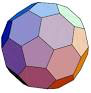
\includegraphics[width=2in]{images/Soccerball.png}
\caption{A faces of a soccer ball are 12 pentagons and 20 hexagons.  Source: \url{http://mathworld.wolfram.com/TruncatedIcosahedron.html}.
}
\label{fig:Soccer}
\end{center}
\end{figure}


\begin{exercise}{Soccer1}
With the help of Figure~\ref{fig:Soccer} determine the number of edges and vertices of the soccer ball. 
\end {exercise}

Let's try to count the rotations of a soccer ball that preserve symmetry.  Axes can be placed through the center of pentagonal faces, which are stabilized in pairs.  Axes can also be placed through the center of hexagonal faces.  However, not all rotations about an axis through a hexagonal face will result in symmetry.

\begin {exercise}{Soccer2}
Let $G$ be the rotation group of a soccer ball. 
\begin{enumerate}[(a)]
\item How many rotations (besides the identity) stabilize at least one pentagonal face? 
\item How many rotations (besides the identity) stabilize at least one hexagonal face?
\end{enumerate}
\end {exercise}

Axes of rotation also pass through edges that join two hexagonal faces. 

\begin{exercise}{Soccer3}
**How many rotations in $G$ (besides the identity) stabilize at least one edge?
\end {exercise}

\begin{exercise}{Soccer4}
\begin{enumerate}[(a)]
\item Find $|G|$ using the counting formula applied to the pentagonal faces.
\item Find $|G|$ using the counting formula applied to the hexagonal faces.
\item Find $|G|$ using the counting formula applied to the edges.
\end{enumerate}
\end{exercise}

\section{Euler's formula for regular polyhedra}
In this section we'll play with counting the order of the rotation group $G$ of a regular polyhedron in different ways. It turns out that this will lead us to an interesting and useful formula relating the number of edges, vertices, and faces in a polyhedron.
Let's start by reviewing our previous examples and noticing a pattern.

\begin {exercise}{Eulers1}
\begin {enumerate}[(a)]
\item
Complete the table and compare $|G|$ to the number of edges of each polyhedron.  The number of edges is equal to the order of the orbit of any edge $e$, denoted as $|{\cal O}_e|$.

\begin{tabular}{|c | c | c|}\hline
polyhedron & number of edges ($|{\cal O}_e|$) & order of group ($|G|$)\\ \hline
cube &  12 &   24\\ \hline
octahedron & -- &--\\ \hline
dodecahedron &  --&--\\ \hline 
\end{tabular}
\item Write an equation for $|G|$ in terms of ${\cal O}_e$.
% $|G|=2\cdot |{\cal O}_e|\$
\end{enumerate}
\end {exercise}
 Now in Exercise~\ref{exercise:actions:Stabilizers2} we showed another way of counting the elements of $G$. Essentially, we showed that we could express $|G|$ as:
\[ |G| = 1 + |\text{stabilizers of faces}| + |\text{stabilizers of vertices}| + |\text{stabilizers of edges}|, \]
where the `1' comes because we need to count the identity.
We'll call this the \bfii {stabilizer counting formula}\index{Stabilizer!counting formula}.

Let's apply this formula to a polyhedron with $|{\cal O}_f|$ faces, $|{\cal O}_v|$ vertices and $|{\cal O}_e|$ edges.  
We'll start with the faces.   For any face $f$ we already have a formula for $|G_f|$  using the counting formula in Proposition~\ref{prop:CountingFormula}. Dividing this formula by $|{\cal O}_f|$ gives:  $|G_f|=|G|/|{\cal O}_f|$.  By substitution we see that $|G_f|=(2\cdot|{\cal O}_e|)/|{\cal O}_f|$. But we know that one of the elements of $|G_f|$ is the identity, which has already been counted.    Since there are $|{\cal O}_f|$ different faces, this\emph{ seems to} imply that there are  $|{\cal O}_f|\cdot (2|{\cal O}_e|/|{\cal O}_f|-1)= 2|{\cal O}_e|-|{\cal O}_f|$ different stabilizers of faces (besides the identity). 

 By the same method, we can count the number of stabilizers of vertices and edges. This gives us $2|{\cal O}_e|-|{\cal O}_v|$ and $2|{\cal O}_e|-|{\cal O}_e|$ stabilizers of vertices and edges, respectively.  Putting these numbers into our stabilizer counting formula we \emph {apparently} get
 \begin{align*}
``|G| &= 1+ 2|{\cal O}_e|-|{\cal O}_f|+ 2|{\cal O}_e|-|{\cal O}_v| +|{\cal O}_e| \\
&= 1+ 5|{\cal O}_e|-|{\cal O}_f|-|{\cal O}_v|''.
\end{align*}
We've put this equation in quotes for a reason.  Let's see if it actually works. 

\begin{exercise}{Eulers2}
Let $G$ be the rotational symmetries of a cube.  Then $|G|=24$.  Verify whether the above formula accurately calculates $|G|$.
\end{exercise}
Something is wrong!  How come we have too many elements?
For all previous examples of polyhedra every element in a rotation group $G$ stabilizes at least two elements of the set $X=\{\text{faces}\}\cup\{\text{edges}\}\cup\{\text{vertices}\}$. For example, In the rotational symmetry group of a cube faces are stabilized in pairs.  This means that we've counted every stabilizer twice. So we need to divide by two in our formula: 
$$|G| = 1+ 5|{\cal O}_e|/2-|{\cal O}_f|/2 -|{\cal O}_v|/2 .$$
Let's see if the stabilizer counting formula works now.

\begin {exercise}{Euler 4}
\begin{enumerate}[(a)]
\item Verify the above equation work for the cube.
\item Verify it works for the tetrahedron.
\item Verify that it works for a soccer ball
\end{enumerate}
\end {exercise}

Let's put this equation together with our expression $|G|=2\cdot |{\cal O}_e|$ to discover a relationship between the number of faces, vertices, and edges of any regular polyhedron:
\begin{align*}
& 2|{\cal O}_e|=1+5|{\cal O}_e|/2-|{\cal O}_f|/2-|{\cal O}_v|/2 \qquad \text{(by substitution)}\\
& |{\cal O}_f|+|{\cal O}_v|-|{\cal O}_e|=2 \qquad \text{(by basic algebra)}\\
\end {align*}
This powerful tool is known as\bfii{ Euler's formula}\index{Euler's formula}.  Let's see how it can be used.

\begin {exercise}{Euler5}
A regular icosahedron has 12 triangular faces and 30 edges.  By Euler's formula, how many vertices does an icosahedron have?
\end {exercise}
We should clarify that what we've shown is only a very special case of Euler's formula which is much more general and has lots of applications in graph theory and topology.  

\section{Closing comments on polyhedral symmetry groups}
Finally we mention that the rotational symmetries of the regular solids are not the only possible symmetries. Recall that in the dihedral group, besides rotations there were reflections. Consider for example the hexagon: it had 6 rotations (including the identity) and 6 reflections. It's possible to rotate the hexagon and keep the hexagon in the same plane. However, to reflect the hexagon, you have to ``flip'' it, which requires three dimensions.  It turns out that something similar is true for the regular solids. There are also reflection symmetries for the regular solids: in fact, there are as many reflections as rotations, just as in the dihedral group. Also like the dihedral group, to reflect a solid requires one extra dimension. It is rather mind-blowing to think that if we lived in a world with four physical dimensions, it would be possible to turn a cube inside out just by moving it!
\section{Group actions on subgroups and cosets}\label{SubgroupsAndCosets}
Let's explore some other examples of group action with applications that we may find familiar.   It turns out that if the set $X$ is also a group, then it's always possible to define a group action of $X$ on itself.

\begin{example}{SubgroupAction1}
Let $X= Z_5$  and $G = Z_5$. Show that in this case, $X$ is a $G$-set.
In order to show that $X$ is a $G$-set we must show $1x = x$ for all $x \in\mathbb {Z}_5$; this is true by identity property of multiplication $\mathbb{Z}_5$.  Then we need to show: $(g_1g_2)x = g_1(g_2x)$ for all $x, g_1,g_2 \in\mathbb{ Z}_5$. This is true by the associative property of multiplication $\mathbb {Z}_5$.  Therefore, by definition of $G$-set, $\mathbb{Z}_5$ is a $G$-set of itself.
\end {example}

\begin {exercise}{SubgroupAction2}
\begin {enumerate} [(a)]
\item Let $X =\mathbb{ Q}^* $ (the nonzero rational numbers) and $G = \mathbb{Q}^*$. Show that in this case, $X$ is a $G$-set.

\item Let $X = H_5$ and $G = H_5$ (The complex 5th roots of unity:  see Section~\ref{sec:RootsOfUnity}  ). Show that in this case, $X$ is a $G$-set.
\item Let $X = T$ (the unit circle in the complex numbers:  see Figure~\ref{rtsunity} in Section~\ref{sec:RootsOfUnity}).  Find a group $G$ such that $X$ is a $G$-set, and prove the statement.
\end{enumerate}
\end {exercise}
We can generalize the results of the preceding exercise in the following proposition:

\begin{prop}{GSetSelf} 
For any group $G$, if we let $X=G$ then $X$ is a $G$-set using the mapping: $(g, x) \rightarrow  gx$.
\end{prop}

\begin {exercise}{GSetSelf2}: 
Prove the above proposition.
\end {exercise}
In the previous exercises, we've seen cases where $X=G$ is a group and $H$ is a subgroup of $X$.  In this situation, $H$ will always produce a group action on $X$.

\begin{exercise}{HSet} 
Prove the following proposition:  If $X=G$ and $G$ is a group, and $H$ is a subgroup of $G$, then $G$ is a $H$-set using the mapping: $(h, g)\rightarrow hg$.
\end {exercise}

Recall our discussion of cosets in Chapter~\ref{cosets} In particular, a left coset consists of a group element $g$ acting on a subgroup $H$ of $G$. The group element acts on each element of the subgroup to create a coset. In other words, a coset is a subgroup shifted by action of a group element.  If $G$ is a group, we can let $L$ be the set of left cosets. We will see in the following examples that we can define a group action on $L$.  That is the set of left cosets, $L$ is a $G$-set.
Let $G$ be the additive group of real numbers.  That is, $G=(\mathbb{R},+)$, and let $H$ be all integer multiples of $2\pi$.   That is, $H=\{2k\pi:k\in \mathbb{Z}\}$, or $H = 2 \pi \mathbb{Z}$ for short.  

\begin{exercise}{AngleCoset1}
Prove that $2 \pi \mathbb{Z}$ is a subgroup of $(\mathbb{R},+)$.
\end{exercise}
\begin {example}{AngleCoset2}
Let $L$ be the set of left cosets of $2\pi \mathbb{Z}$ in the group $(\mathbb{R},+)$.  Recall from Definition~\ref{def_coset} in Chapter~\ref{cosets} that the set of left cosets $L$ is defined as $x+2\pi \mathbb{Z}=\{x+h:h\in 2\pi\mathbb{Z}\}$.  For example, the left coset which contains $\pi/3$ is the set $ \{\pi/3 +2k\pi, k\in \mathbb{Z}\}$, which we could also write as $\{ \ldots \pi/3-4\pi, \pi/3-2\pi, \pi/3, \pi/3+2\pi, \pi/3 + 4\pi, \ldots \}$.  It turns out that $L$ is $G$-set under the action  
$(g,x+2\pi\mathbb{Z}) \rightarrow g+x+2\pi\mathbb{Z}$. Let's verify the two axioms (conditions) of a $G$-set:
\begin{enumerate}[(a)]
\item
 For the first axiom note that $e\in G=0$. Then, $0+x+2\pi\mathbb{Z}=x+2\pi\mathbb{Z}$ for any $x+2\pi\mathbb{Z}\in L$.  So the first axiom is true.
\item 
For the second axiom consider two real numbers $a,b$.  Then, by associativity of real number addition, $(a+b)+x+2\pi\mathbb{Z}=a+(b+x+2\pi\mathbb{Z})$ for any $x+2\pi\mathbb{Z}$  in $L$.  So the second axiom is true.  $L$ is a $G$-set of the additive group of real numbers.
\end {enumerate}
This example has a very practical significance. We know that angles on a unit circle are arbitrary up to multiples of $2\pi$. So we can think of each angle as a coset:  that is, the angle $\theta$ where $0\leq\theta<2\pi$ represents the coset $\{\theta +2k\pi\}$ or $\theta + 2\pi \mathbb{Z}$. Now consider what an arbitrary rotation $\phi$ does to the angle $\theta$. For instance, consider the case where $\theta=\frac{\pi}{4}$--then $\theta+H=\{ \frac{\pi}{4}+2k\pi\}$.  We'll suppose that the rotation angle is $\phi=\frac{15\pi}{2}$.  According to the group action, $\phi+\theta+H =\frac{15\pi}{2}+\{\frac{\pi}{4}+2k\pi\}$ which will result in the new coset $\{\frac{31\pi}{4}+2k\pi\}=\{\frac{7\pi}{4}+2k\pi\}$.
As we can see, the action of the additive group $(R,+)$ on the cosets ${\theta + 2\pi k}$ corresponds to rotation by arbitrary angles around the unit circle. If the rotation is more than $2 \pi$, the action still works because the cosets take care of any extra factors of $2 \pi$.
\end {example}
Let's consider another example of group action on a set of cosets.  This example can be thought of as a two-dimensional version of the previous example, and can be envisioned using computer graphics.

\begin {example}{IntLat1}
Let $G$ be the $xy$ plane under addition (that is, $G=(\mathbb {R}^2,+)$).  Let $H=\mathbb{Z}\times \mathbb{Z}$, which is a subgroup of $G$ ($H$ is called the \bfii{integer lattice}\index{Integer!lattice}).  
A coset of $H$ in $G$ is defined as $x+H=\{(x+m, y+n):m,n \in\mathbb{ Z}\}$
Each coset of the form $x+H$ has a single point inside the unit square.
Consider, $g=(0.2,0), x=(0.9,0.5)$ and  $h=(m,n)$, for $g,x\in G$ and $h\in H$.
  $g+x+H={(0.2+.9+m, 0+0.5+n):m, n \in Z}={(1.1+m, 0.5+n):m, n \in Z}$
Using $h= (-1, 0)$ yields $g+x+h=(0.1, 0.5)$, the single point for the coset $g+x+H $ which is inside the unit square.
$g+x+H$ is equivalent to the coset $(0.1, 0.5)+H$ 
Imagine the unit square is your computer screen.  The example above can be used to describe the motion of a character on the screen of a “wraparound'' video game.  That is, if he moves off the right edge of the screen, he re-appears on the left edge as shown in Figure~\ref{fig:UnitSquare}. 
\end{example}

\begin{figure}[ht]
\begin{center}
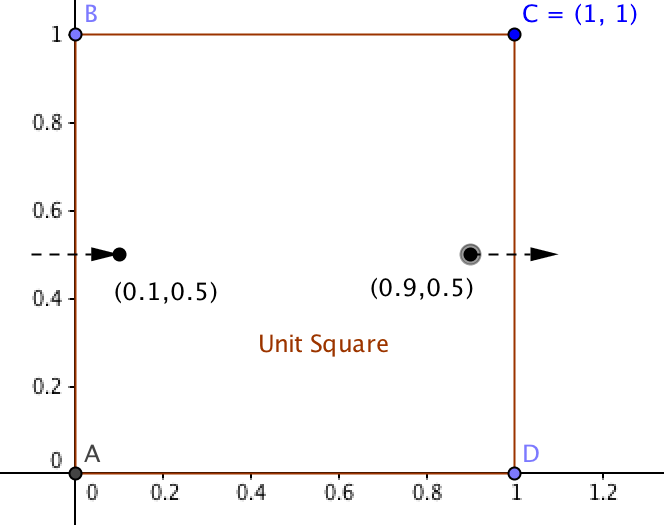
\includegraphics[width=3in]{images/UnitSquare.png}
\caption{Unit square illustrating a left group action of $G=(\mathbb {R}^2,+)$ on the left cosets of $H=\text{integer lattice}$ in $G$ }
\label{fig:UnitSquare}
\end{center}
\end{figure}

Recall that by definition a left coset of the integer lattice $x+H$  means adding the same point $\{x=(a,b)|a,b\in \mathbb{R}\}$ to each point in the integer lattice. a group action simply changes one coset of $H$ in $G$ to a different coset.  The three illustrations below show the progression of the group action  in the Example~\ref{example:actions:IntLat1}. You can duplicate this illustration by drawing the coset points on a transparency, placing it over a graph of the integer lattice and moving the transparency $0.2$ units to the right.

\begin{figure}[ht]
\begin{center}
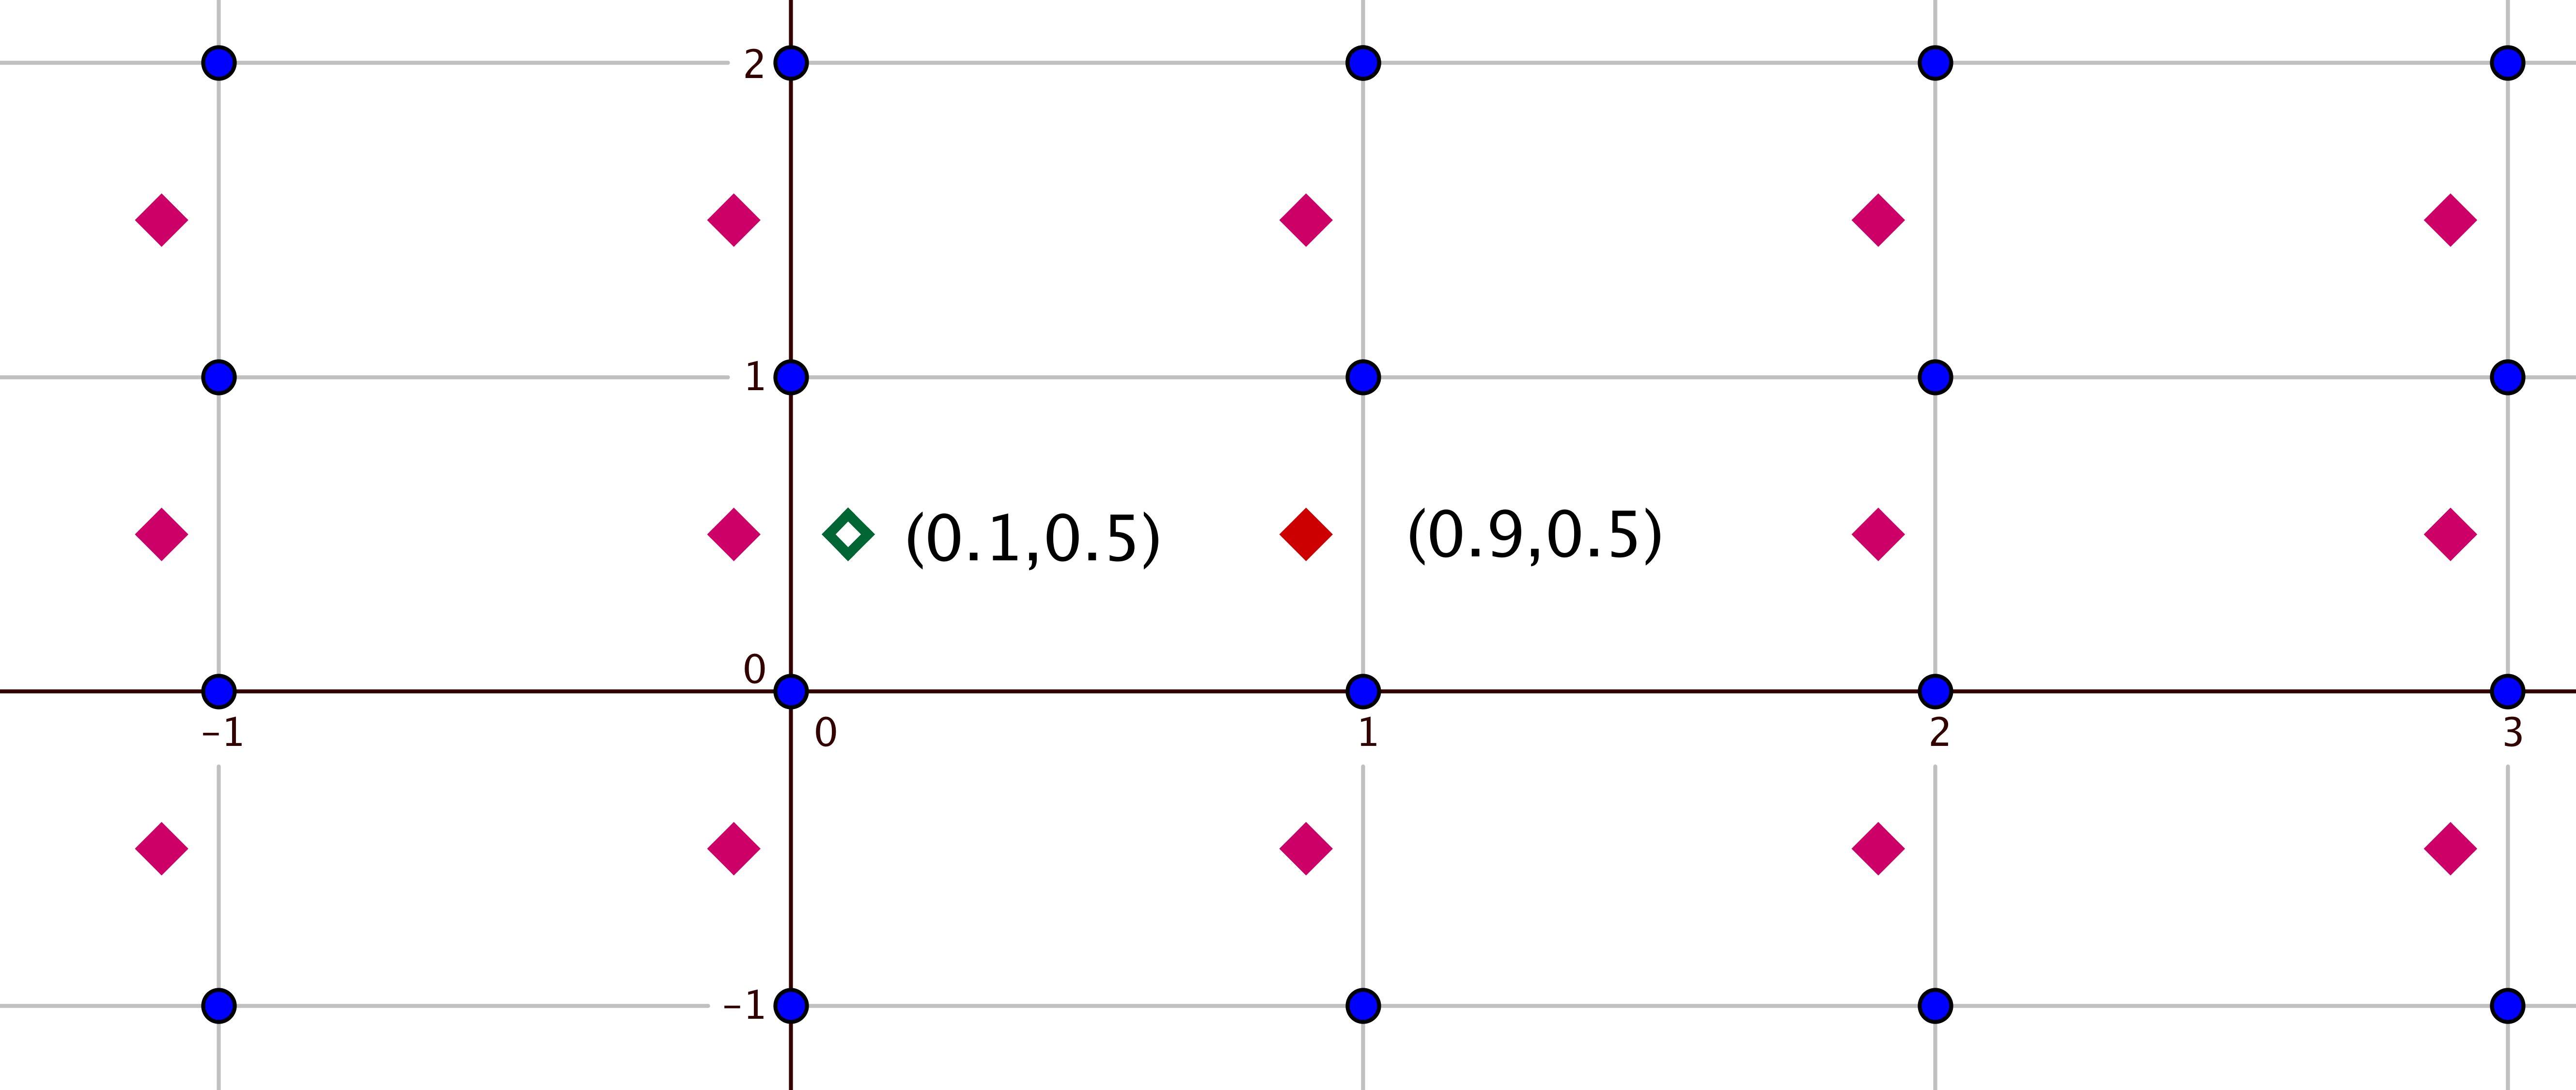
\includegraphics[width=4.0in]{images/IntLat1.png}
\caption{Illustrating $x+H$ for $x=(0.9,0.5)$ Note: this illustration and the two following were created using the software ``GeoGebra'' (see \url{www.geogebra.org}).  
The rectangles should be thought of as unit squares (the scales on the $x$ and $y$ axes are not equal).   These figures illustrate a left group action of $(\mathbb{R},+)$ on a left coset of integer lattice.}
\label{fig:IntegerLattice1}
\end{center}
\end{figure}

\begin{figure}[ht]
\begin{center}
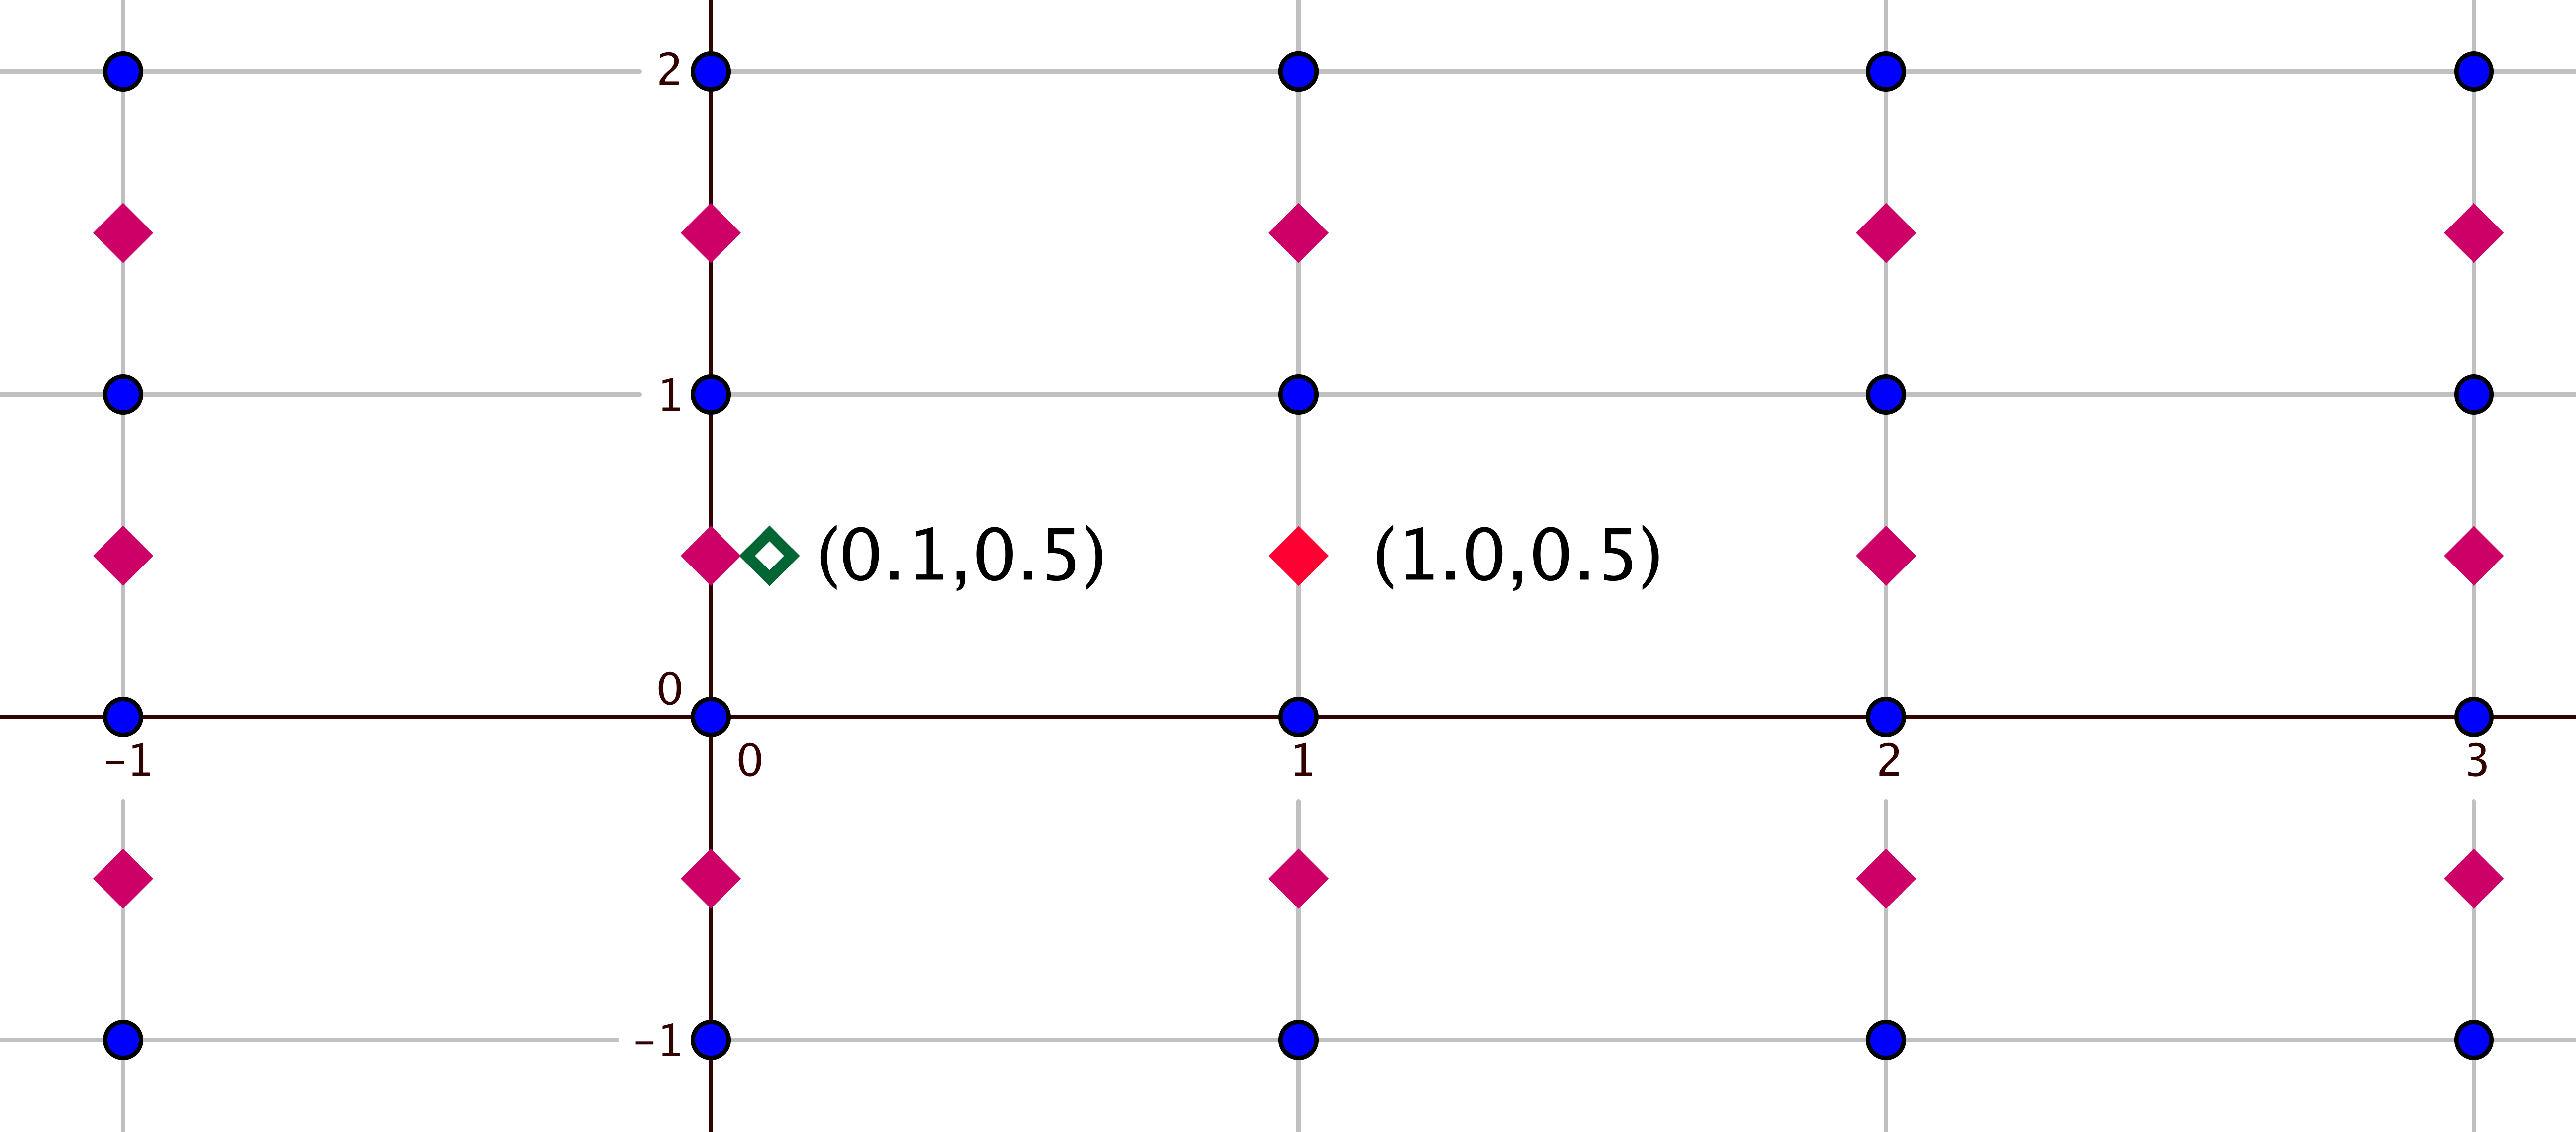
\includegraphics[width=4.0in]{images/IntLat2.png}
\caption{Illustrating $g+x+H$ for $g=(0.1,0)$ and $x=(0.9,0.5)$}
\label{fig:IntegerLattice2}
\end{center}
\end{figure}


\begin{figure}[ht]
\begin{center}
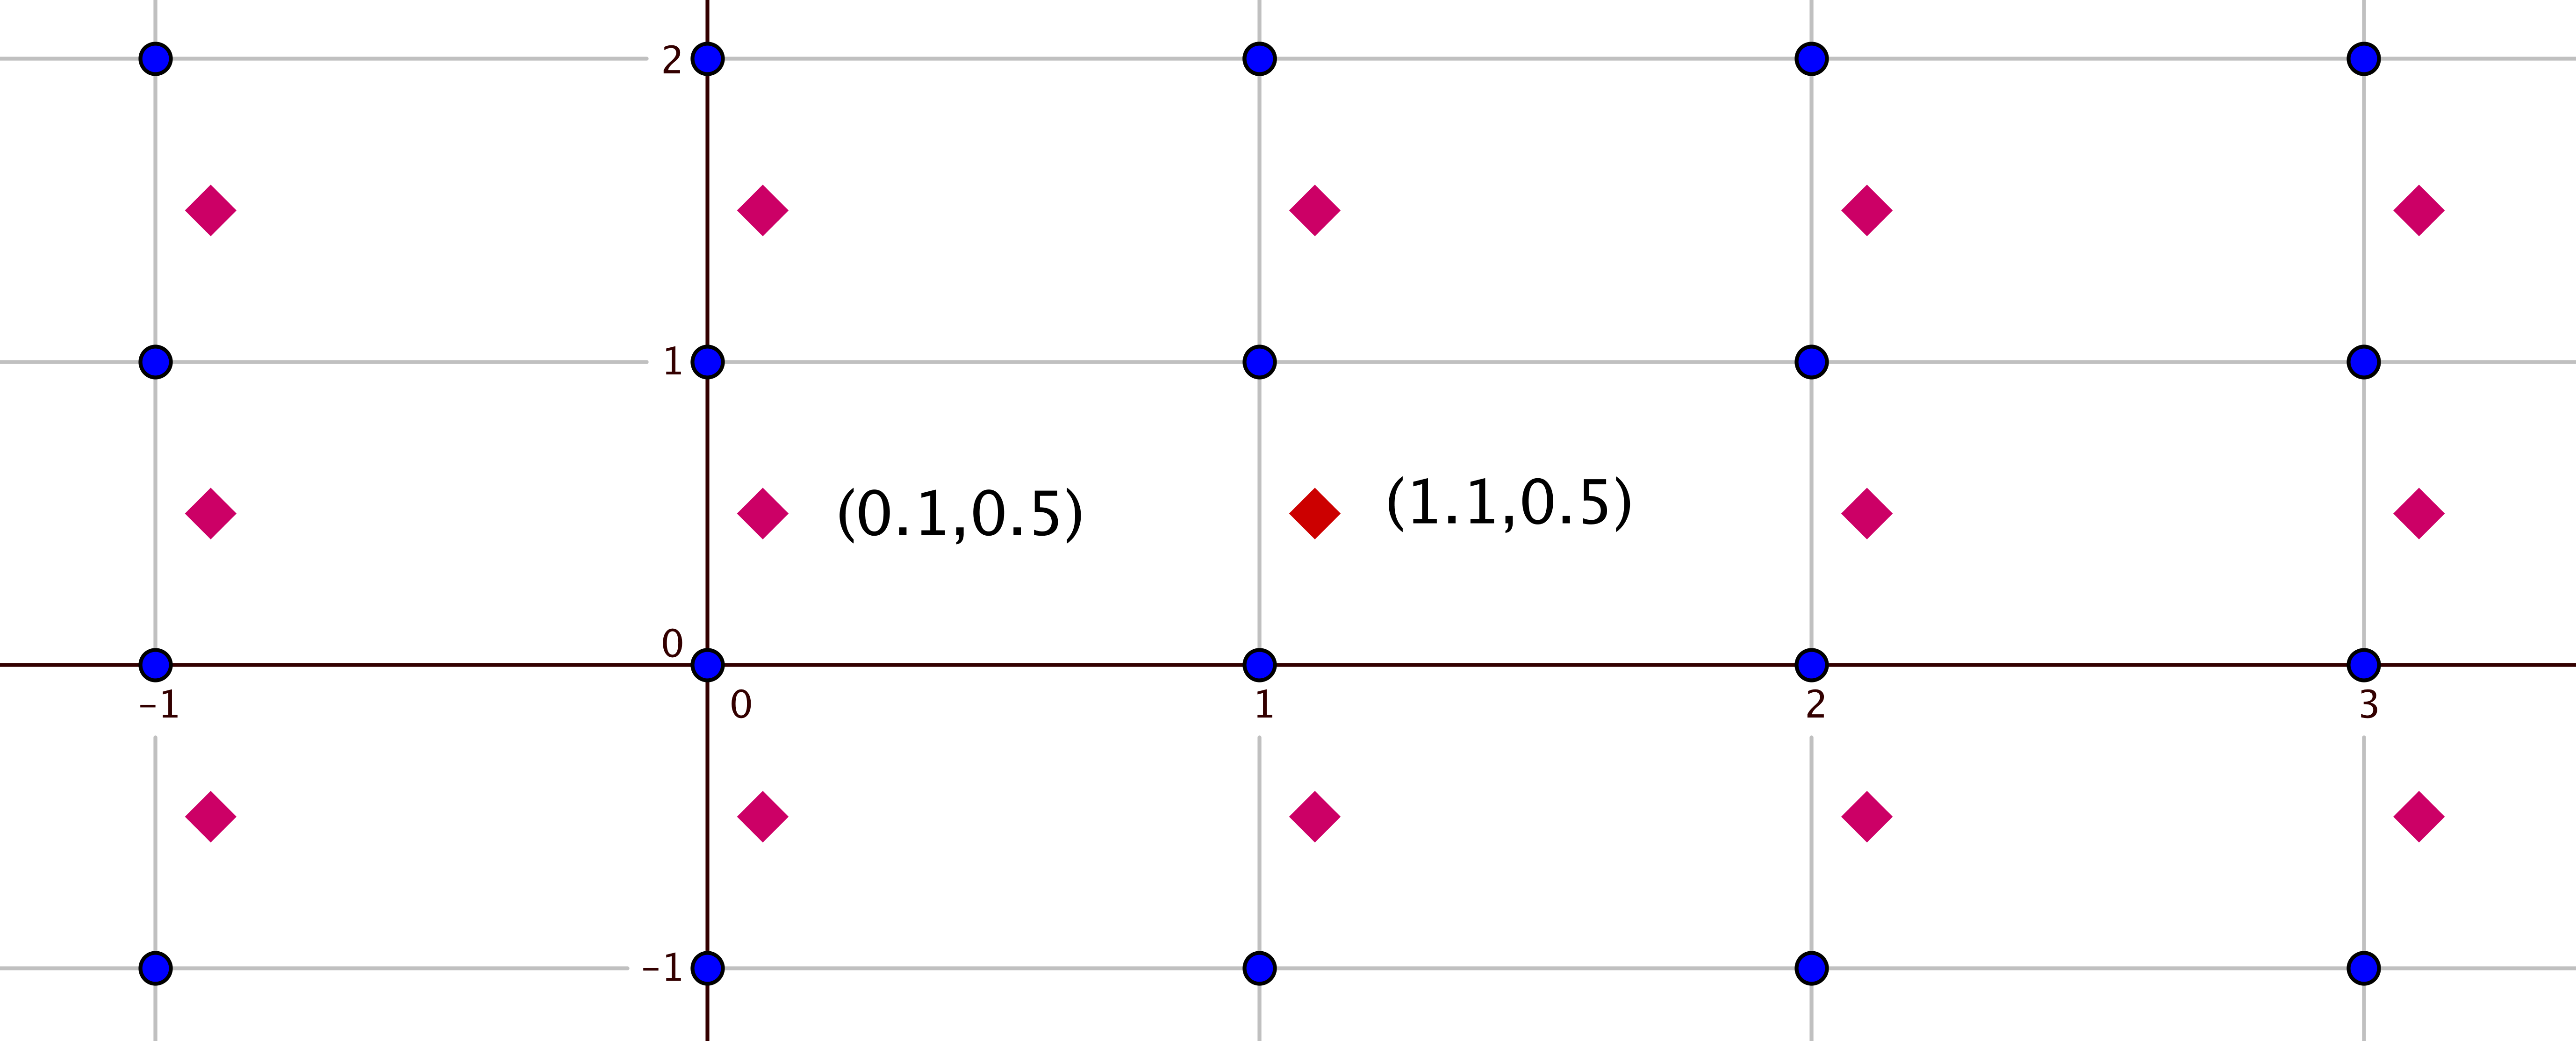
\includegraphics[width=4.0in]{images/IntLat3.png}
\caption{Illustrating $g+x+H$ for $g=(0.2,0)$ and $x=(0.9,0.5)$}
\label{fig:IntegerLattice3}
\end{center}
\end{figure}


\begin {exercise}{IntLat2}
\begin {enumerate}[(a)]
\item Given $x=(0.8,0.6)$ and $g=(1.4,0)$ find a point  $h\in \mathbb{Z}\times \mathbb{Z}$ Such that $g+x+h$ is inside the unit square.  (In fact, this is the \emph{only} point $h$ for which $g+x+H$ is inside the unit square.)
\item Given $x=(0.8,0.6)$ and $g=(1.2,1.3)$ find a point  $h\in \mathbb{Z}\times \mathbb{Z}$ Such that $g+x+h$ is inside the unit square.
\item Given $x=(0.8,0.6)$ and $g=(0,3.5)$ find a point  $h\in \mathbb{Z}\times \mathbb{Z}$ Such that $g+x+h$ is inside the unit square.
\item For each $g$ and $x$ above, find $g'$ in the unit square, such that $g'+H=g+x+H$.
\item Illustrate part (a) with a graph.  Graph the point $x$.  (This is actually the point $x+h'$ for $h'=(0,0)$).  Then graph the point $g+x+h$ using the $h$ you found in part (a).   Include ordered pairs to indicate the position of points.  Include arrows to indicate ``movement'' as in the example.
\item Create a similar graphs illustrating part (b) and (c).
\item Prove that the above are examples of a group action of $G$ on $x+H$.  That is, show that $x+H$ is a $G$-set. 
\end{enumerate}
\end {exercise}
We can think about this example in another way.  Suppose we have a \emph{torus}, which is the mathematical word for a donut shape. We could imagine creating a ``map'' of the surface of the torus by cutting the torus apart as shown in Figure~\ref{fig:Torus1}. If we spread this map out flat, it would look like a square (see Figure~\ref{fig:Torus2}). If we wanted to use the map to chart motion on the surface of the torus, then any motion that goes off the right edge would reappear at the left edge; and any motion that goes off the top edge would reappear at the bottom.  So you see this is exactly what we saw for the previous example. So using cosets of $\mathbb{Z}^2$ in $\mathbb{R}^2$, we've created a mathematical representation for motion on the surface of a torus.

\begin{figure}[ht]
\begin{center}
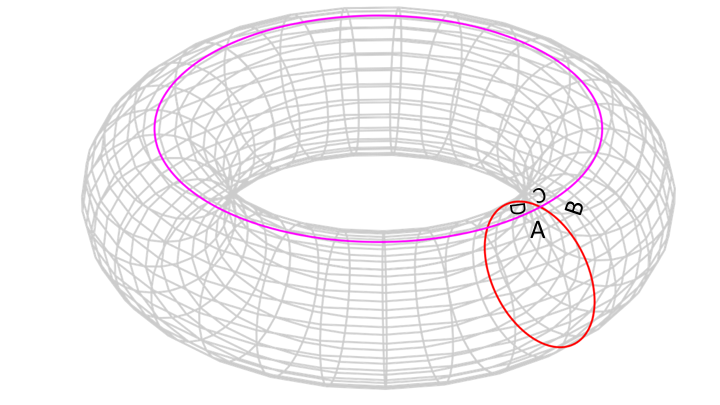
\includegraphics[width=3in]{images/Torus1.png}
\caption{Torus, showing two cut lines.}\label{fig:Torus1}
\end{center}
\end{figure}

\begin{figure}[ht]
\begin{center}
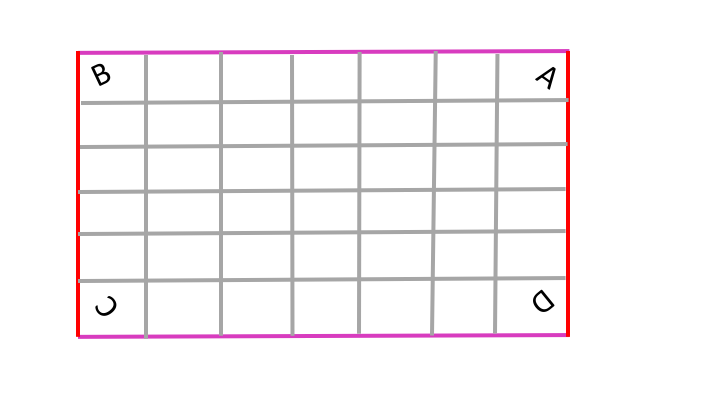
\includegraphics[width=3in]{images/Torus2.png}
\caption{The cut torus, flattened out.}\label{fig:Torus2}
\end{center}
\end{figure}

We can generalize the two previous examples by considering cosets of a subgroup $H$ in a group $G$ that contains $H$.

\begin{example}{CosetAction}
Let $H$ be a subgroup of $G$ and $L_H$ the set of left cosets of $H$. The set $L_H$ is a $G$-set under the action 
$(g,xH)\rightarrow gxH$.
Again, it is easy to see that the first axiom is true. Since $(gg')xH = g(g'xH)$, the second axiom is also true.
\end{example}
So far, we've been looking at group actions on left cosets.  What about right cosets?  Let's investigate.

\begin {exercise}{RtCosetAction}
Consider the case where $G=S_3$, $H=\{\var{id},(12)\}$, and $R$ is the set of right cosets of $H$.  Define a function from $G\times R\rightarrow R$ by $(g,R)\rightarrow Rg$. Does this function define a group action of $G$ on $R$? 
\hyperref[sec:actions:hints]{(*Hint*)}
\end {exercise}
The previous exercise shows that we can't always do the same thing with right cosets that we can do with left cosets.  Let's look at an alternative:  

\begin {exercise}{RtCosetAction2}
\begin{enumerate}[(a)]
\item Repeat the previous exercise, but this time use the function $(g,R)\rightarrow Rg^{-1}$.
\item Show that in general the function $(g,R)\rightarrow Rg^{-1}$ defines an action of $G$ on the right cosets of $H$.  
\end {enumerate}
\end {exercise}
\section{Conjugation}\label {Conjugation}
\subsection*{Commutative diagrams and the definition of conjugation}
When we talked about permutations, we saw that the objects we were permuting didn't really change the situation.  For example, we saw that permuting $\{1,2,3,4\}$ was the ``same thing'' as permuting $\{A,B,C,D\}$. Now what do we really mean by the ``same thing''? Well for example, if we take any permutation of $\{1,2,3,4\}$ and replace $1$ with $A$, $2$ with $B$ and so on, then we'll get a permutation of $\{A,B,C,D\}$. To be specific let's take $\sigma=(123)$ and $f=\begin {pmatrix} 1&2&3&4\\A&B&C&D\end {pmatrix}$.  It's possible to represent this situation with diagram in Figure~\ref{fig:Commutative1}. This type of diagram is called a \bfii{commutative diagram}.\index{Commutative!diagram}


The commutative diagram illustrates the construction of a conjugation. We can begin in the upper right corner and travel to the upper left, in the opposite direction of the $f$ arrow. That is $f^{-1}$.  Then, from upper left to lower left represents the permutation $\sigma=(123)$.  Then, proceed in the direction of the arrow, that is $f$ from lower left to lower right.  At the lower right corner, we arrive at the mapping of $\mu$.  So the diagram shows $\mu=f\sigma f^{-1}$.  (Recall functions are composed from right to left.).  

\begin{figure}[ht]
\begin{center}
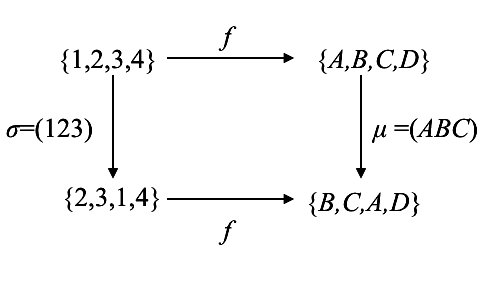
\includegraphics[width=2.5in]{images/Commutative1.png}
\caption{Commutative diagram of a conjugate mapping.}\label{fig:Commutative1}
\end{center}
\end{figure}

Let's think of this another way. We can follow the path $f\sigma$ or $\mu f$.  Both take us to the lower right. 
 So we can write $f\sigma$= $\mu f$. By right multiplying by $f^{-1}$ we discover the algebraic structure of the conjugate of $\sigma$,  $f\sigma f^{-1}=\mu$.  
There is a short cut to arrive at $\mu$.  $\mu$ is simply $\sigma$ relabeled according to $f$.  That is, if we take the cycle representation of $\sigma$ and replace the numbers according to $f$ ($1\rightarrow A, 2\rightarrow B, 3\rightarrow C$), then we end up with $\mu$.  We will call this short cut, ``the relabeling method''.\index{Conjugation!relabling method}

\begin{exercise}{Conj1}
For each $\sigma$ and and $f$, complete a commutative diagram like the one in Figure~\ref{fig:Commutative1}. Find the conjugate mapping in two ways, using conjugation and the relabeling method.
\begin{enumerate}[(a)]
\item $\sigma=(12)(35)$ and $f=\begin{pmatrix} 1&2&3&4&5\\ A&B&C&D&E& \end{pmatrix} $
\item $\sigma=(2346)$ and $f=\begin{pmatrix} 1&2&3&4&5&6\\ A&B&C&D&E&F \end{pmatrix}$
\item $\sigma=(147)(2563)$ and $f=\begin{pmatrix} 1&2&3&4&5&6&7\\ A&B&C&D&E&F&G \end{pmatrix}$
\end{enumerate}
\end {exercise}
Now instead of $f$ going between different sets, we can choose $f$ to map $\{1,2,3,4\}$ to itself. In this case, $f$ itself is a permutation.  To be more consistent with our earlier notation for permutations, we'll use the symbol $\tau$ instead of $f$ in the following discussion.  What $\tau$ corresponds to is just relabeling the objects that we're permuting. Figure~\ref{fig:Commutative2} shows an example where both $\tau$ and $\sigma$ are permutations on the set $\{1,2,3,4\}$. The diagram shows that if we do a permutation $\sigma$ on the originally-labeled objects, and compare to the same permutation of the relabeled objects, we find that the relabeled permutation is exactly given by $\tau\sigma \tau^{-1}$. The permutations $\sigma$ and $\tau\sigma \tau^{-1}$ are called \bfii{conjugate permutations}\index{Permutation!conjugate}, and the operation which takes $\sigma$ to $\tau \sigma \tau^{-1}$ is called \bfii{conjugation}.\index{Conjugation!of permutations}\footnote{Note this is quite different from conjugation of complex numbers. Unfortunately, ``conjugation'' is a very popular word in mathematics, and is used in many different senses.}

\begin{figure}[ht]
\begin{center}
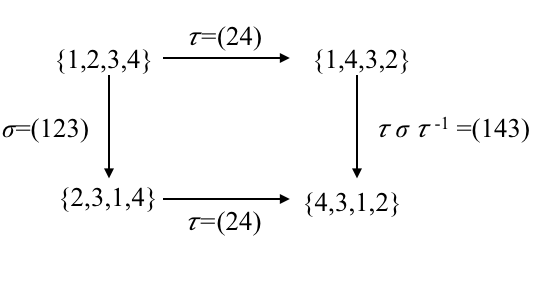
\includegraphics[width=3in]{images/Commutative2.png}
\caption{Conjugate mapping with $\tau$ and $\sigma$ permuting \{1,2,3,4\}.}\label{fig:Commutative2}
\end{center}
\end{figure}

\subsection *{Conjugate permutations and cycle structure}

Two permutations that are conjugate are in many ways very similar. We could almost call them the ``same'' permutation, only they act on a relabeled set of objects. In particular, it's true that two conjugate permutations must have the same cycle structure. For instance, in the example we did earlier in Figure~\ref{fig:Commutative1} we saw that both permutations were three-cycles.  This will be true in general because conjugation simply means relabeling the objects that are permuted, without changing anything else.

\begin{example}{Conj2}
Let $\sigma = (153)(276)$ and $\tau = (427)(165)$. Then
$$\tau=\begin{pmatrix} 1&2&3&4&5&6&7\\6&7&3&2&1&5&4  \end{pmatrix}.$$ 
Relabeling $\sigma$ according to $\tau$ gives the conjugate $(136)(457)$. You can check that computing $ \tau \sigma \tau^{-1}$ will give the same result as the relabeling method.
\end{example}
\begin{exercise}{Conj3}
Given $\sigma$ and $\tau$ use the relabeling method to find the permutation conjugate to $\sigma$.  Check your work by computing the conjugate with $\tau\sigma\tau^{-1}$
\begin{enumerate}[(a)]
\item $\sigma=(6247)$ and $\tau=(527)(63)$.  $\sigma$ and $\tau$ act on the set $\{1,2,3,4,5,6,7\}$.
\item$\sigma=(256)(134)$ and $\tau=(21643)$.  $\sigma$ and $\tau$ act on the set $\{1,2,3,4,5,6\}$.
\item$\sigma=(14)(27356)$ and $\tau=(463)$.  $\sigma$ and $\tau$ act on the set $\{1,2,3,4,5,6,7\}$.
\end{enumerate}
\end{exercise}

It turns out that it's also true that any two permutations with the same cycle structure are conjugate.

\begin{example}{Coj4}
Let $\sigma = (12)(3456)(789), \mu = (149)(2658)(37)$.  Notice that $\sigma$ becomes $\mu$ if we use the following relabeling:
$$ 1 \rightarrow 3;~~2 \rightarrow 7;~~3\rightarrow 2;~~4\rightarrow 6;~~5\rightarrow 5;~~6\rightarrow 8;~~7\rightarrow 1;~~8\rightarrow 4;~~9\rightarrow 9.$$
We can use this information to write $\tau$ in tableau notation:
$$ \tau =\begin{pmatrix} 1&2&3&4&5&6&7&8&9 \\ 3&7&2&6&5&8&1&4&9 \end{pmatrix}, $$
from which we find, $\tau=(1327)(468)$.  Then you may check that $\sigma$ and $\mu$ are conjugate according to: $\mu = \tau \sigma \tau^{-1}$.
\end{example}
\begin{exercise}{Conj5}
In each of the following find a permutation $\tau$ that makes $\sigma$ and $\mu$ conjugate.  Check that $\sigma$ and $\mu$ are conjugate according to: $\mu = \tau \sigma \tau^{-1}$.

\begin {enumerate}[(a)]
\item $\sigma=(135)(792)(468)$, $\mu=(236)(189)(457)$
\item $\sigma=(2579)(3561)$, $\mu=(2461)(5793)$
\item $\sigma=(25)(13578)$, $\mu=(36)(28454)$
\end{enumerate}
\end{exercise}
These examples lead up to the following theorem:

\begin{prop}{ConjPerm} Given a permutation group $G$, and two permutations $\sigma, \mu \in G$.  Then $\sigma$ and $\mu$ are conjugate if and only if they have exactly the same cycle structure.
\end{prop}
\begin{proof}
The ``only if'' part follows from remarks we have made above: the conjugation operation simply re-labels the elements of the permuted set, so two conjugate permutations must have the same cycle structure.
For the ``only if'' part, we may write $\sigma$ in cycle notation as
$$\sigma = (a¬_{11}~a_{12}~\ldots~a_{1n_1})(a¬_{21}~a_{22}~\ldots~a_{2n_2})  \ldots(a¬_{k1}~a_{k2}~\ldots~a_{k n_k}).$$  
Suppose that $\tau$ has the same cycle structure, which means that $\tau$ can be written as
$$\tau = (b¬_{11}~b_{12}~\ldots~b_{1n_1})(b¬_{21}~b_{22}~\ldots~b_{2n_2})  \ldots(b_{k1}~b_{k2}~\ldots~b_{k n_k}).$$
Then we can define a bijection $f$ by: $f(a_{ij}) = b_{ij}$, for any $i$ and $j$. Using the above cycle structures, we can show that $\tau$ is equal to $f \sigma f^{-1}$.  All we have to do is show that this works for any $ b_{ij}$.  For example, consider $b_{11}$: then $f \sigma f^{-1}( b_{11}) = f \sigma ( a_{11}) = f ( a_{12})= b_{12}$, which is exactly equal to $ \tau(b_{11})$.
\end{proof}

\subsection*{Conjugacy and group action}

We will now relate the idea of conjugacy with the notion of group action that was introduced earlier in the chapter.


\begin{example}{Conj6}
Let $G$ be the dihedral group $D_4$.  Recall that $D_4$ consists of four rotations and four reflections.  In fact we can write $D_4=\{e, r, r^2, r^3, s,s\compose r,s\compose r^2,s\compose r^3\}$, where $r$ is counterclockwise rotation by $90^{\circ}$, and $s$ is the reflection that leaves vertices labeled $1$ and $3$ fixed.  Let $H$ be the subgroup $\{e,s\}$.  
We'll define our mapping from $H\times G \rightarrow G$ as follows:
$$(h,g) \rightarrow hgh^{-1}. $$
For example, consider the case $h=s$ and $g=r$. Then $(s,r) \rightarrow s\compose r \compose s^{-1}$.  We can simplify this, since $s$ is a reflection, so $s^{-1}=s$.  furthermore, by part c of Proposition~\ref{proposition:symmetries:Dn_generator_theorem}  in Section~\ref{sec:dihedral}, we can show $r\compose s =s\compose r^3$.  This gives us
$$ s\compose r\compose s^{-1}=s\compose r\compose s=s\compose s\compose r^3=r^3.$$

\end {example}
\begin{exercise}{Conj7}
Complete the previous example with $G=D_4$ and $H=\{e,s\}$ by listing all the pairs $(h,g)$ with $h\in H$ and $g \in G$ together with the result of the mapping $hgh^{-1}$.  Simplify your expression for $hgh^{-1}$ as much as possible.
\end{exercise}
Note something very interesting in the previous exercise.  When $h=e$ the all elements of $G$ remain unchanged by the mapping, but when $h=s$ all the rotations map to their inverses.
% at the end of the chapter add an exercise that relates conjugation to change of basis in linear algebra. 
 We can generalize Example \ref{example:actions:Conj6} using the following definition.

\begin{defn}
Given two group elements $g,h$ in $G$, then $hgh^{-1}$ is said to a \bfii{conjugate element}\index{Conjugate!element} to $g$. In this case, we would say that $h$ acts on $g$ by conjugation.\index{Conjugation!operation on groups}
\end{defn}
%try to come up with another example of conjugation
The definition of conjugation gives us a new group action for any subgroup $H$ acting on a group $G$ which contains $H$:

\begin{prop}{HSetCojugation}. If $H$ is a subgroup of $G$, then $G$ is an $H$-set under conjugation.  That is, we can define an action $H \times G\rightarrow G$, by $(h, g) \rightarrow hgh^{-1}$ for $h\in H$ and $g\in G$. 
\end{prop}
The proof is contained in the following exercise.

\begin{exercise}{Conj8}
Fill in the blanks to proof the proposition:

\noindent
First, we have that $\underline{~<1>~}$ is in  $H$ and $(e, g) = \underline{~<2>~}g\underline{~<3>~} = g$.
So the first axiom for a group action holds. 

Also, observing that
\[(h_1h_2,g) = \underline{~<4>~}g\underline{~<5>~}
= h_1(h_2g\underline{~<6>~} )\underline{~<7>~}
= (h_1, (\underline{~<8>~}, g)),\]
we see that the second condition is also satisfied.
\end{exercise}

%First, we have that \underline{e} is in  $H$ and $(e, g) = \underline{e}g\underline{e}^{-1} = g$.
%So the first axiom for a group action holds. 

%Also, observing that
%
%\[(h_1h_2, g) = \underline{h_1h_2}g(\underline{h_1h_2})^{-1}
%= h1(h2g\underline{h_2} ^{- 1})\underline{h_1}^{-1}
%= (h1, (\underline{h_2}, g)),\]

\subsection*{Order of conjugate elements}

In order to illustrate some properties of the action of conjugation, we will take a familiar example: the group of rotational symmetries of a cube.
What are the conjugate elements?
We've seen that the rotations can be classified into:
\begin{itemize}
\item
Stabilizers of faces;
\item
Stabilizers of vertices;
\item
Stabilizers of edges;
\item
Stabilizers of everything (identity).
\end{itemize}
Which of these are conjugate? 


Consider the conjugates of $r_z$, which is a 90 degree counterclockwise rotation around the $z$ axis. Supposing that $g$ is an arbitrary rotational symmetry, what does $g r_z g^{-1}$ do? First, the $g^{-1}$ will rotate another pair of faces to the top and bottom positions. Then, $r_z$ will rotate that pair of faces by 90 degrees. Then $g$ will rotate the two rotated faces back to their original places. The net result will always be a 90 degree rotation of an opposite pair of faces of the cube. 
The question now is, are \emph{all} such 90 degree rotations conjugate to each other? In particular, are 90 degree \emph{counterclockwise} rotations the same as 90 degree \emph{clockwise} rotations? For instance, is $r_z$ conjugate to $r_z^{-1}$.  In fact it is, as we'll see in the next example.

\begin {example}{Conj9} 
Let  $g=r_x^2$ then consider $r_x^2\compose r_z\compose r_x^{-2}$ .   What will this rotation do? First $r_x^{-2}$ will take the top face to the bottom face and vice versa. Then $r_z$ will rotate the face $z_-$ (which is now on top)  90 degrees counterclockwise and  $z_+$ (which is now on the bottom) 90 degrees clockwise.  Then $r_x^2$ will rotate $z_-$ back to the bottom and $z_+$ back to the top.  So we see $r_x^2\compose r_z\compose r_x^{-2} = r_z^{-1}$. (This is related to the formula $s r s^{-1} = r^{-1}$, which we saw in Chapter~\ref{symmetries}.)  
\end{example}

We have also seen that it's possible to rotate any pair of opposite faces to the top and bottom face. This means that any 90 rotation of any pair of opposite faces of the cube is conjugate to $r_z$.  

\begin {exercise}{Conj10}
\begin {enumerate} [(a)]
\item In view of Exercise~\ref{exercise:symmetries:InverseRot} of Chapter~\ref{symmetries}, what's another way to write $r_z^{-1}$ ?  
\item What rotation results from the composition  $r_y^2\compose r_x^3\compose r_y^{-2}$?
\item What is the order of each of the following: $r_x^3, r_x, r_z, r_z^{-1}$? 
\end{enumerate}
\end{exercise}

The order of rotations plays an important role in determining which group elements are conjugate:

\begin {exercise}{Conj11}
\begin {enumerate}[(a)]
\item What is the result of the following conjugation? $r_x\compose r_z^2 \compose r_x^{-1}$
\item Will a rotation conjugate to $r_z^2$ ever have order 4?  Explain your answer.
\end {enumerate}
\end{exercise}

We've seen that stabilizers of faces are conjugate to each other if they are rotations of the same order.  Let's consider stabilizers of vertices.

\begin {example}{Conj12}
 $r_y\compose r_z$ is a 120 degree stabilizer of vertex {+\,+\,+}.  Consider the conjugation of $r_y\compose r_z$ by the group element $r_y$, that is,  $r_y\compose (r_y\compose r_z)\compose r_y^{-1}$. First, $r_y^{-1}$ takes ${+\,+\,-}$ to ${+\,+\,+}$.  Then $r_y\compose r_z$ rotates ${+\,+\,-}$ 120 degrees counterclockwise. Then $r_y$ rotates ${+\,+\,-}$ back to its original place.  The net result is a 120 degree counterclockwise rotation of the vertex ${+\,+\,-}$.
\end{example}

\begin{exercise}{Conj13}
\begin{enumerate}[(a)]
\item Which vertex does $r_z\compose r_y$ stabilize?  What is the order of this stabilizer?  
\item Consider the conjugate $r_x^{2}\compose (r_z\compose r_y)\compose r_x^{-2}$.  Which vertex will this stabilize?  What is the order of this stabilizer?
\item What is the order of a conjugate of a stabilizer of a  cube's vertex?  Is the order always the same?  Explain your answer.
\end {enumerate}
\end {exercise}

Finally, let's consider  conjugates of stabilizers of edges.

\begin{example}{Conj14}
The rotation $r_z^2\compose r_y^{-1}$ stabilizes the edge $\overline{x_- z_-}$.  It's a 180 degree rotation about an axis through this edges  $\overline{x_- z_-}$ and $\overline{x_+z_+}$. Consider the conjugate   $r_z^{2}\compose (r_z^2\compose r_y^{-1})\compose r_z^{-2}$.  What does this rotation do?  First,  $r_z^{-2}$ takes $\overline{x_+z_-}$ to $\overline{x_-z_-}$.  Then $(r_z^2\compose r_y^{-1})$ rotates about the axis through $\overline{x_+z_-}$ 180 degrees, switching the two faces. Then $r_z^2$ rotates $\overline{x_+z_-}$ back to its original position.  The net result is a 180 degree rotation about the axis through $\overline{x_+z_-}$ and $\overline{x_-z_+}$.
\end{example}

\begin{exercise}{Conj15}
\begin{enumerate}[(a)]
\item The rotation $y^2\compose z$ stabilizes the edge $\overline{x_+y_+}$. One conjugate of this rotation $r_y\compose (y^2\compose z)\compose r_y^{-1}$ What does the conjugate stabilize?
\item What is the order of a conjugate of a stabilizer of an edge of a cube? Is the  order always the same?  Explain your answer.
\end {enumerate}
\end{exercise}

For all the examples we've seen so far, the order of a conjugate of any stabilizer is the same as the order of the stabilizer itself. Of course, examples are not proof--but in this case they're a strong indication that this may be a general property. In fact, we can show: 

\begin{thm} Let $G$ be a group, $g \in G$, and $\tilde{g}$ is conjugate to $g$. Then $|g| = |\tilde{g}|$: that is,  $g$ has the same order as $\tilde{g}$.
\end{thm}

\begin{proof}  The proof is outlined in the following exercise.

\begin{exercise}{Conj15b}
Fill in the blanks to complete the proof that a group element and its conjugate always have the same order.

Suppose that $\tilde{g}$ is conjugate to $g$. This means that there exists an $x\in G$ such that $\tilde{g}=\underline{~<1>~}$. Suppose $|g|=n$. Compute $\tilde{g}^n$ as follows:
\begin{align*}
 \tilde{g}^n&=(\underline{~<2>~}) \ldots (\underline{~<4>~})~~~~~~~~~n~\text{ times)}\\ 
& =xg(\underline{~<5>~})g \ldots g(\underline{~<6>~})gx^{-1}\qquad\text{(associative property)}\\
&=xg(\underline{~<7>~})g...g(\underline{~<8>~})gx^{-1}=x(\underline{~<9>~})x^{-1}=\underline{~<10>~}\quad\text{( inverse property)}
\end{align*}
\noindent
It follows that  $| \tilde{g}| \leq |\underline{~<11>~}|$. On the other hand, \[(\underline{~<12>~})\tilde{g}(\underline{~<13>~})=g\qquad\text{(inverse property)}.\]  
The same proof shows that $|g|\underline{~<14>~}|\tilde{g}|$ Therefore,  $|g|=\underline{~<15>~}$ 
\end {exercise}
\end{proof}

\begin{exercise}{Conj15c}
We've shown that if elements are conjugate they must have the same order.
\begin {enumerate}[(a)]
\item What is the converse of the above statement?
\item Prove or disprove the converse using previous examples to help you.
\end{enumerate}
\end {exercise}
 
%In summary the stabilizers of the different faces are either 90  degree rotations (order 4) or 180 degree rotations (order 2) (as we've seen above, 270 degree counterclockwise rotations can be counted as 90 degree clockwise rotations). All of these 90 degree rotations are conjugate, and all 180 degree rotations are conjugate.  Since stabilizers of vertices are 120 or 240 degree rotations (both order 3) these stabilizers are conjugate to each other.  Also the 180 degree (order 2) rotations of about axes through edges are conjugate to each other.  

\subsection*{Conjugacy classes and the class equation}

We have seen before that $g$-equivalent elements form an equivalence class. This means that the operation of conjugacy defines an equivalence relation, and every set of conjugate elements is an equivalence classes. These equivalence classes are known as \bfii{conjugacy classes}.\index{Conjugacy!class}
The upshot is that we have the group $G$ partitioned into 5 conjugacy classes, consisting of: 
\begin{itemize}
\item
the identity, 
\item
90 degree stabilizers of faces, 
\item
180 degree stabilizers of faces, 
\item
stabilizers of vertices, 
\item
stabilizers of edges. 
\end{itemize}

This is exactly the method we used before to count up the number of elements in $G$.  
What we've just done for the rotational symmetries of a cube can be done for any group.  We have the general formula:
$$|G| = \sum (\text{orders of conjugacy classes}).$$
This is known as the \bfii{class equation}.\index{Class equation}

\begin{example}{Conj15}
  We can verify that the class equation correctly calculates the order of the group of rotational symmetries of a cube. 

\begin{align*}
|G|=&|\text{conjugacy class of 90 degree stabilizers of faces}| \\
&~+|\text{conjugacy class of 180 degree stabilizers of faces}|\\
&~+|\text{conjugacy class of stabilizers of vertices}|\\
&~+|\text{conjugacy class of stabilizers of edges}|\\
&~+|\text{conjugacy class of identity}|\\
=&6+3+8+6+1\\
=&24.
\end{align*}
\end{example}

Let's use the class equation to verify $|G|$ for some other familiar groups.  

\begin {example}{Conj16}

Consider the group $S_3$.  Note this is the same as the dihedral group of an equilateral triangle.  
Let $s$ be the reflection that leaves the vertex labeled `1' fixed, and let $r$ be the counterclockwise rotation by 120 degrees.  We can find the conjugacy classes of $S_3$ by creating a table with a column for each of the elements in the group.  Each row will represent a conjugacy class.  

It's clear that $\var{id}$ has its own conjugacy class of one element.  For example, 
$r^2\compose \var{id} \compose r=r^2\compose r=\var{id}$. We can verify that $\var{id}$ is only conjugate to itself.

 We can see that $r$ has two conjugates.  For example:

 $\var{id}\compose r \compose \var{id}=r$ 

$s\compose r \compose s=s\compose s\compose r^2=\var{id}\compose r^2=r^2$
by Proposition~\ref{proposition:symmetries:Dn_generator_theorem}  in Chapter~\ref{symmetries}.  

% We can complete the rows for $\var{id}$ and $r$.
%
%\begin{tabular}{|r | c | c |c | c | c |c |}\hline
%$g$ &$\var{id}$ & $r$ &$r^2$ &$ s$ &$ s\compose r$ & $s\compose r ^2$\\ \hline
%$g\compose \var{id}\compose g^{-1}$ & $\var{id}$ & $\var{id}$ & $\var{id}$ &$\var{id}$ &$\var{id}$ &$\var{id}$ \\ \hline
%$ g\compose r\compose g^{-1}$& $r$&$ r$& $r$&$r^2$ &$r^2$ & $r^2$\\ \hline
%\end {tabular} 


We don't need a row for $r^2$ because it belongs to the same conjugacy class as $r$.  
Computing the row for $s$ completes the table, since $s$ is conjugate to all the other reflections.

\begin{center}
\begin{tabular}{|r | c | c |c | c | c |c |}\hline
$g$ &$\var{id}$ & $r$ &$r^2$ &$ s$ &$ s\compose r$ & $s\compose r ^2$\\ \hline
$g\compose \var{id}\compose g^{-1}$ & $\var{id}$ & $\var{id}$ & $\var{id}$ &$\var{id}$ &$\var{id}$ &$\var{id}$ \\ \hline
$ g\compose r\compose g^{-1}$& $r$&$ r$& $r$&$r^2$ &$r^2$ & $r^2$\\ \hline
$g\compose s\compose g^{-1}$ & $s$ &$ s\compose r$ & $s\compose r^2$ & $s$ & $s\compose r^2$ & $s\compose r$\\ \hline 
\end{tabular}
\end{center}

%\emph{Note}: We don't need anymore rows in the table since $s$ is conjugate to each of the reflections.  So, all reflections are in the same conjugacy class.

The table shows that $S_3$ is partitioned into  three conjugacy classes: $\var{id}$, rotations and reflections of orders 1, 2, and 3 respectively.  The class equation verifies the order of $S_3$.

$|S_3|=1+2+3=6$
\end{example}

\begin {exercise}{Conj17}
\begin {enumerate}[(a)]
\item Complete a conjugacy table like the one in  Example~\ref{example:actions:Conj16} for $G=D_4$. As in the example $r$ is a counterclockwise rotation by 90 degrees and $s$ is the reflection that leaves the vertex labeled "1" fixed. Compute and simplify the conjugate expressions as compositions of $r$ and $s$. We show one row.  How many more rows are needed to complete the table?

\begin{center}

\begin{tabular}{ |r| c | c |c |c |c |c | c|c |} \hline
  $g$ &$\var{id}$ & $r$ &$r^2$ &$r^3$ & $s$ &$s\compose r$ & $s\compose r ^2$ & $s\compose r^3$\\ \hline
  $g\compose \var{id}\compose g^{-1}$ &--- & -- & -- &-- &--&--&--&-- \\
\end{tabular}
\end{center}

 Remember, once a group element appears in a row, you don't need to compute a row for that element, because you have already found its conjugacy class.
\item Verify that the class equation correctly calculates $|D_4|$.
\end{enumerate}
\end{exercise}

\begin {example}{Conj 18}
We can also create a conjugacy table for using permutation notation. Here is the conjugacy table for $S_3$ using permutations.
  
\begin{center}
\begin{tabular}{|r | c | c |c | c | c |c |}\hline
$g$ &$(1)$ & $(123)$ &$(132)$ & $(23)$ & $(13)$ & $(12)$\\ \hline
$g\compose (1)\compose g^{-1}$ &$(1)$ & $(1)$ & $(1)$ &$(1)$ &$(1)$ & $(1)$ \\ \hline
$ g\compose (123)\compose g^{-1}$& $(123)$&$(123)$& $(123)$&$(132)$ &$(132)$ & $(132)$\\ \hline
$g\compose(23)\compose g^{-1}$ & $(23)$ &$(13)$ & $(12)$ & $(23)$ & $(12)$ & $(13)$\\ \hline 
\end{tabular}
\end{center}

Recall the relabeling method in Exercise  ~\ref{exercise:actions:Conj3}.  We recommend using this method to save time when making conjugacy tables.  

For instance, to simplify $(12)\compose (23)\compose (12)$ we can relabel (23) according to (12).  That is: $2\rightarrow 1$ and $3\rightarrow 3$.  So,  $(12)\compose (23)\compose (12)=(13)$.
\end{example}

In the next exercise you may practice creating a conjugacy table using both permutation notation and the relabeling method.

\begin{exercise}{Conj 19}
\begin{enumerate}[(a)]
\item Create a conjugacy table for $A_4$ (The subgroup of even permutations in $S_4$) See Definition~\ref {Alternating_Group} of Section~\ref{sec:AlternatingGroup}. We show one a table with one row.  How many rows to complete the conjugacy table? (Use the relabeling method to save time in creating your table.)

\begin{center}
\begin{tabular}
{|r |c| c| c| c| c|c}\hline
 $x$& $(1)$& $(12)(34)$&$(13)(24)$&$(14)(23)$&$(123)$&\ldots\\ \hline
$g \compose(1)\compose g^{-1}$ & -- & --& --&--&--& \ldots \\ 
\end{tabular}
\end{center}

\item Verify that the class equation correctly calculates $|A_4|$.
\end {enumerate}
\end {exercise}


%Let $G=A_4$ Recall from Definition~\ref{Alternating_Group} of Section~\ref{The alternating group} That $A_4$ is the subgroup of even permutations of $S_4$.  Also note by Proposition~\ref{proposition:permute:Alternating1} of ~\ref{section:permute:The Alternating Group} that $| A_n | = n!/2$.  All of $A_4$ is made up of  even permutations. 
% In $A_4$ what are the conjugates of $(12)(34)$?  We can make a table of $x\compose (12)(34)\compose x^{-1}$ for all x in $A_4$:
%

%
%\end{tabular}
%\end {example}
%
%\begin {exercise}{Conj20}
%Let $G$ be the group $D_4$ 
%\begin{enumerate}
%

\begin {exercise}{Conj21}
Let $G$ be an abelian group of finite order and $x,g\in G$.
Simplify the conjugate expression $x\compose g\compose x^{-1}$.  How many conjugacy classes are in the abelian group $G$? How many elements are in each conjugacy class? 
\end{exercise}


